\documentclass[]{book}
\usepackage{lmodern}
\usepackage{amssymb,amsmath}
\usepackage{ifxetex,ifluatex}
\usepackage{fixltx2e} % provides \textsubscript
\ifnum 0\ifxetex 1\fi\ifluatex 1\fi=0 % if pdftex
  \usepackage[T1]{fontenc}
  \usepackage[utf8]{inputenc}
\else % if luatex or xelatex
  \ifxetex
    \usepackage{mathspec}
  \else
    \usepackage{fontspec}
  \fi
  \defaultfontfeatures{Ligatures=TeX,Scale=MatchLowercase}
\fi
% use upquote if available, for straight quotes in verbatim environments
\IfFileExists{upquote.sty}{\usepackage{upquote}}{}
% use microtype if available
\IfFileExists{microtype.sty}{%
\usepackage[]{microtype}
\UseMicrotypeSet[protrusion]{basicmath} % disable protrusion for tt fonts
}{}
\PassOptionsToPackage{hyphens}{url} % url is loaded by hyperref
\usepackage[unicode=true]{hyperref}
\hypersetup{
            pdftitle={Comparative Methods Workshops},
            pdfauthor={Chris Mitchell},
            pdfborder={0 0 0},
            breaklinks=true}
\urlstyle{same}  % don't use monospace font for urls
\usepackage{natbib}
\bibliographystyle{apalike}
\usepackage{color}
\usepackage{fancyvrb}
\newcommand{\VerbBar}{|}
\newcommand{\VERB}{\Verb[commandchars=\\\{\}]}
\DefineVerbatimEnvironment{Highlighting}{Verbatim}{commandchars=\\\{\}}
% Add ',fontsize=\small' for more characters per line
\usepackage{framed}
\definecolor{shadecolor}{RGB}{248,248,248}
\newenvironment{Shaded}{\begin{snugshade}}{\end{snugshade}}
\newcommand{\KeywordTok}[1]{\textcolor[rgb]{0.13,0.29,0.53}{\textbf{#1}}}
\newcommand{\DataTypeTok}[1]{\textcolor[rgb]{0.13,0.29,0.53}{#1}}
\newcommand{\DecValTok}[1]{\textcolor[rgb]{0.00,0.00,0.81}{#1}}
\newcommand{\BaseNTok}[1]{\textcolor[rgb]{0.00,0.00,0.81}{#1}}
\newcommand{\FloatTok}[1]{\textcolor[rgb]{0.00,0.00,0.81}{#1}}
\newcommand{\ConstantTok}[1]{\textcolor[rgb]{0.00,0.00,0.00}{#1}}
\newcommand{\CharTok}[1]{\textcolor[rgb]{0.31,0.60,0.02}{#1}}
\newcommand{\SpecialCharTok}[1]{\textcolor[rgb]{0.00,0.00,0.00}{#1}}
\newcommand{\StringTok}[1]{\textcolor[rgb]{0.31,0.60,0.02}{#1}}
\newcommand{\VerbatimStringTok}[1]{\textcolor[rgb]{0.31,0.60,0.02}{#1}}
\newcommand{\SpecialStringTok}[1]{\textcolor[rgb]{0.31,0.60,0.02}{#1}}
\newcommand{\ImportTok}[1]{#1}
\newcommand{\CommentTok}[1]{\textcolor[rgb]{0.56,0.35,0.01}{\textit{#1}}}
\newcommand{\DocumentationTok}[1]{\textcolor[rgb]{0.56,0.35,0.01}{\textbf{\textit{#1}}}}
\newcommand{\AnnotationTok}[1]{\textcolor[rgb]{0.56,0.35,0.01}{\textbf{\textit{#1}}}}
\newcommand{\CommentVarTok}[1]{\textcolor[rgb]{0.56,0.35,0.01}{\textbf{\textit{#1}}}}
\newcommand{\OtherTok}[1]{\textcolor[rgb]{0.56,0.35,0.01}{#1}}
\newcommand{\FunctionTok}[1]{\textcolor[rgb]{0.00,0.00,0.00}{#1}}
\newcommand{\VariableTok}[1]{\textcolor[rgb]{0.00,0.00,0.00}{#1}}
\newcommand{\ControlFlowTok}[1]{\textcolor[rgb]{0.13,0.29,0.53}{\textbf{#1}}}
\newcommand{\OperatorTok}[1]{\textcolor[rgb]{0.81,0.36,0.00}{\textbf{#1}}}
\newcommand{\BuiltInTok}[1]{#1}
\newcommand{\ExtensionTok}[1]{#1}
\newcommand{\PreprocessorTok}[1]{\textcolor[rgb]{0.56,0.35,0.01}{\textit{#1}}}
\newcommand{\AttributeTok}[1]{\textcolor[rgb]{0.77,0.63,0.00}{#1}}
\newcommand{\RegionMarkerTok}[1]{#1}
\newcommand{\InformationTok}[1]{\textcolor[rgb]{0.56,0.35,0.01}{\textbf{\textit{#1}}}}
\newcommand{\WarningTok}[1]{\textcolor[rgb]{0.56,0.35,0.01}{\textbf{\textit{#1}}}}
\newcommand{\AlertTok}[1]{\textcolor[rgb]{0.94,0.16,0.16}{#1}}
\newcommand{\ErrorTok}[1]{\textcolor[rgb]{0.64,0.00,0.00}{\textbf{#1}}}
\newcommand{\NormalTok}[1]{#1}
\usepackage{longtable,booktabs}
% Fix footnotes in tables (requires footnote package)
\IfFileExists{footnote.sty}{\usepackage{footnote}\makesavenoteenv{long table}}{}
\usepackage{graphicx,grffile}
\makeatletter
\def\maxwidth{\ifdim\Gin@nat@width>\linewidth\linewidth\else\Gin@nat@width\fi}
\def\maxheight{\ifdim\Gin@nat@height>\textheight\textheight\else\Gin@nat@height\fi}
\makeatother
% Scale images if necessary, so that they will not overflow the page
% margins by default, and it is still possible to overwrite the defaults
% using explicit options in \includegraphics[width, height, ...]{}
\setkeys{Gin}{width=\maxwidth,height=\maxheight,keepaspectratio}
\IfFileExists{parskip.sty}{%
\usepackage{parskip}
}{% else
\setlength{\parindent}{0pt}
\setlength{\parskip}{6pt plus 2pt minus 1pt}
}
\setlength{\emergencystretch}{3em}  % prevent overfull lines
\providecommand{\tightlist}{%
  \setlength{\itemsep}{0pt}\setlength{\parskip}{0pt}}
\setcounter{secnumdepth}{5}
% Redefines (sub)paragraphs to behave more like sections
\ifx\paragraph\undefined\else
\let\oldparagraph\paragraph
\renewcommand{\paragraph}[1]{\oldparagraph{#1}\mbox{}}
\fi
\ifx\subparagraph\undefined\else
\let\oldsubparagraph\subparagraph
\renewcommand{\subparagraph}[1]{\oldsubparagraph{#1}\mbox{}}
\fi

% set default figure placement to htbp
\makeatletter
\def\fps@figure{htbp}
\makeatother

\usepackage{booktabs}
\usepackage{amsthm}
\makeatletter
\def\thm@space@setup{%
  \thm@preskip=8pt plus 2pt minus 4pt
  \thm@postskip=\thm@preskip
}
\makeatother

\title{Comparative Methods Workshops}
\author{Chris Mitchell}
\date{2020-06-23}

\begin{document}
\maketitle

{
\setcounter{tocdepth}{1}
\tableofcontents
}
\chapter{Preamble}\label{preamble}

This book contains a series of workshops on the use of phylogenetically
controlled comparative methods. The workshops assume a basic familiarity
with R. You should revisit the material from LIFE223 if you need a quick
refresher on R.

\chapter{Introduction}\label{intro}

\chapter{Workshop 1: Plotting phylogenies in R}\label{w1plotting}

\section{Phylogenetics in R}\label{phylogenetics-in-r}

From LIFE223, you know R as a powerful statistical tool. You will also
be aware that it is an incredibly flexible tool for plotting data. In
this workshop, we will be working with phylogenies in R and manipulating
them to produce informative plots.

\subsection{Packages used}\label{packages-used}

In this tutorial we'll mostly be using a package called ggtree. To
install it, we need another package called BiocManager.

\begin{Shaded}
\begin{Highlighting}[]
\KeywordTok{install.packages}\NormalTok{(}\StringTok{"BiocManager"}\NormalTok{)}
\NormalTok{BiocManager}\OperatorTok{::}\KeywordTok{install}\NormalTok{(}\StringTok{"ggtree"}\NormalTok{)}
\KeywordTok{library}\NormalTok{(ggtree)}
\end{Highlighting}
\end{Shaded}

We will also need to use phylobase, ggimage and it would help to have
the tidyverse packages loaded since we'll be using the syntax of
ggplot2. If you get an error message, make sure the packages are
installed first.

\begin{Shaded}
\begin{Highlighting}[]
\KeywordTok{library}\NormalTok{(tidyverse)}
\KeywordTok{library}\NormalTok{(phylobase)}
\KeywordTok{library}\NormalTok{(ggimage)}
\end{Highlighting}
\end{Shaded}

\section{Importing your tree}\label{importing-your-tree}

Let's start by importing a tree. Make sure your working directory is set
to wherever you have saved the tree\_newick file. If you run this line,
you should see an object called ``tree'' appear in your global
environment.

\begin{Shaded}
\begin{Highlighting}[]
\NormalTok{tree <-}\StringTok{ }\KeywordTok{read.tree}\NormalTok{(}\StringTok{"tree_newick.nwk"}\NormalTok{)}
\end{Highlighting}
\end{Shaded}

If we take a look at the structure of our tree object using the
\textbf{str} function. The tree is stored as an object of class
\textbf{phylo}.

\begin{Shaded}
\begin{Highlighting}[]
\KeywordTok{str}\NormalTok{(tree)}
\end{Highlighting}
\end{Shaded}

\begin{verbatim}
List of 4
 $ edge       : int [1:24, 1:2] 14 15 16 17 18 19 20 20 19 18 ...
 $ edge.length: num [1:24] 4 13 10 3 8 6 4 4 5 6 ...
 $ Nnode      : int 12
 $ tip.label  : chr [1:13] "A" "B" "C" "D" ...
 - attr(*, "class")= chr "phylo"
 - attr(*, "order")= chr "cladewise"
\end{verbatim}

We can see a list of 4 elements of the tree object. The first
(\textbf{edge}) contains the edges (also known as branches) of the
phylogeny and their labels. The next is \textbf{edge.length} which
contains the lengths of the branches. \textbf{Nnode} specifies the
number of nodes and finally \textbf{tip.label} contains the labels of
the tips. In this case, we just have letters for tip labels.

Things become clearer when we plot the tree. We can do this with the
\textbf{plot} function in base R.

\begin{Shaded}
\begin{Highlighting}[]
\KeywordTok{plot}\NormalTok{(tree)}
\end{Highlighting}
\end{Shaded}

\begin{center}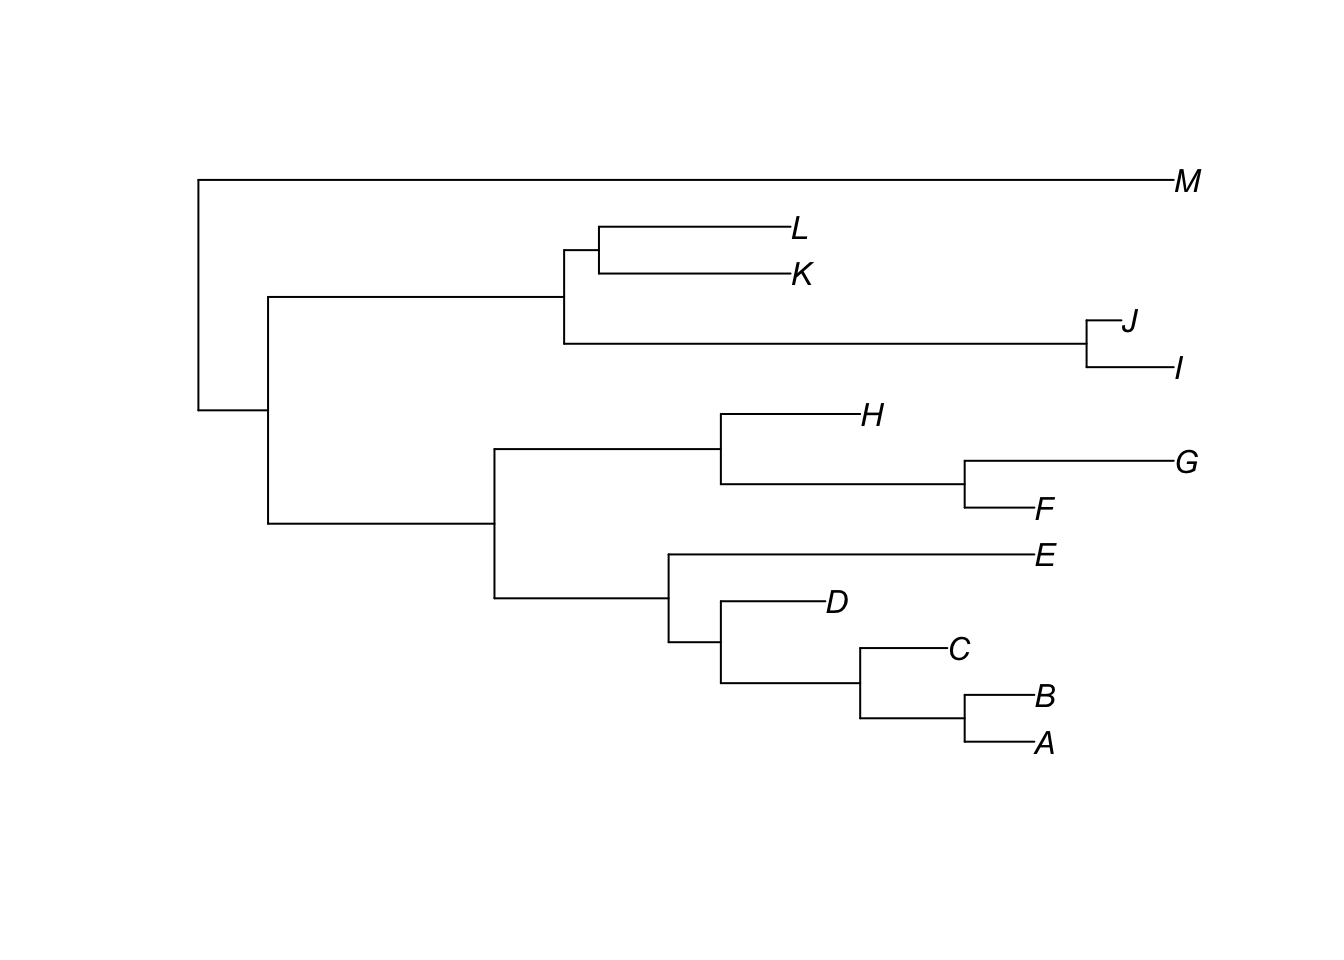
\includegraphics{bookdown-demo_files/figure-latex/unnamed-chunk-7-1} \end{center}

This plot is fine for a quick check to make sure the tree looks as we
expected it to. Let's look at making a more attractive plot with ggtree.

\section{ggtree}\label{ggtree}

The syntax we'll be using here is a little different that what you may
be used to so don't get intimidated. \textbf{ggtree} uses the same
syntax as a package called \textbf{ggplot2}. This works by creating
layers (known as \textbf{geoms}) and plotting them over each other.

We'll start by using ggtree to plot our tree. This is the base layer of
the plot.

\begin{Shaded}
\begin{Highlighting}[]
\KeywordTok{ggtree}\NormalTok{(tree)}
\end{Highlighting}
\end{Shaded}

\begin{center}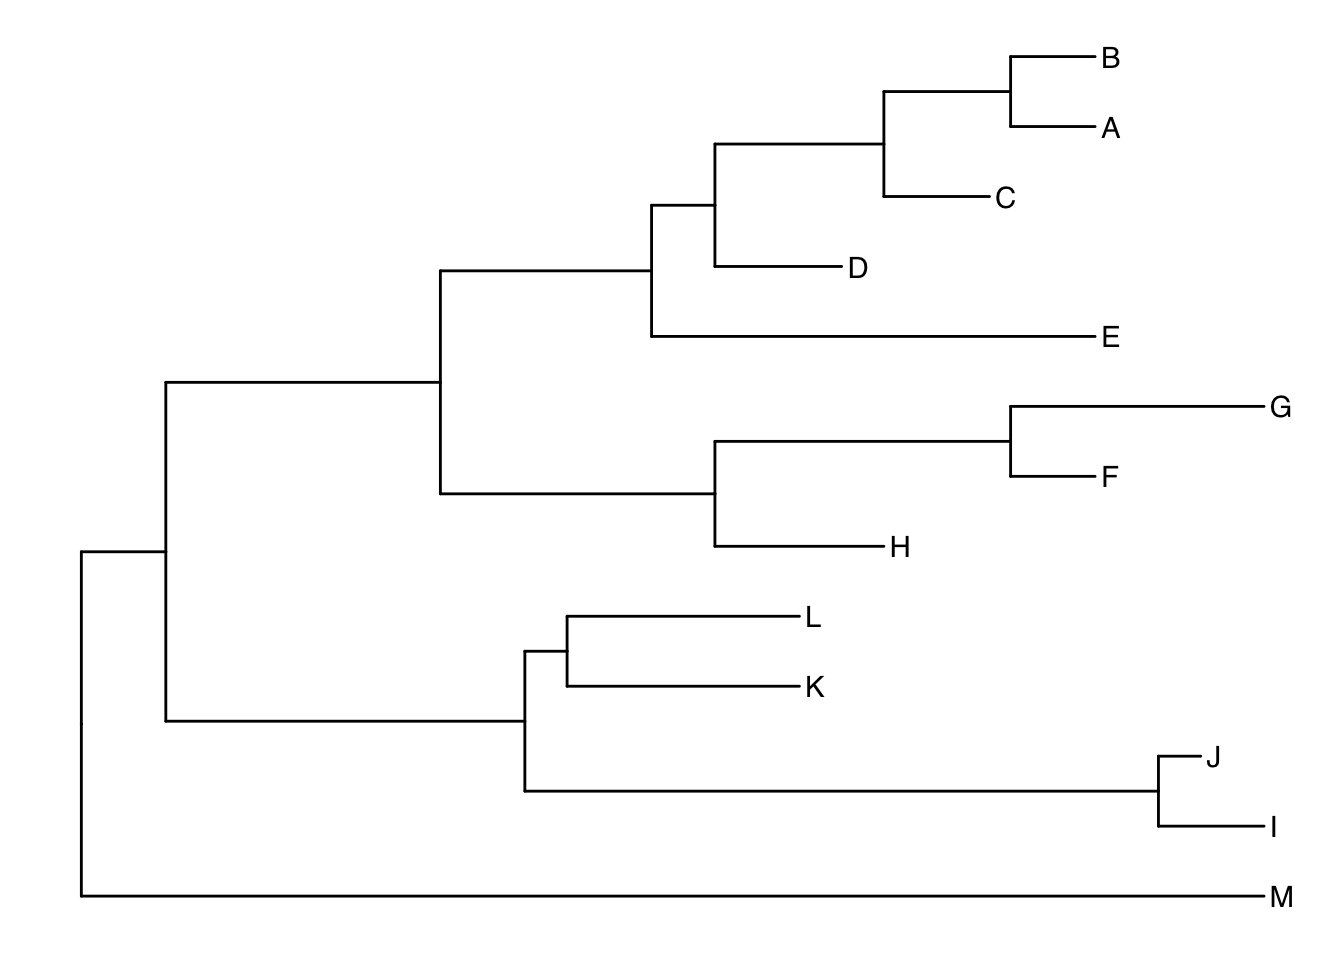
\includegraphics{bookdown-demo_files/figure-latex/unnamed-chunk-8-1} \end{center}

You may want to plot the same tree as a \textbf{cladogram}. To do this,
disable branch lengths.

\begin{Shaded}
\begin{Highlighting}[]
\KeywordTok{ggtree}\NormalTok{(tree, }\DataTypeTok{branch.length =} \StringTok{"none"}\NormalTok{)}
\end{Highlighting}
\end{Shaded}

\begin{center}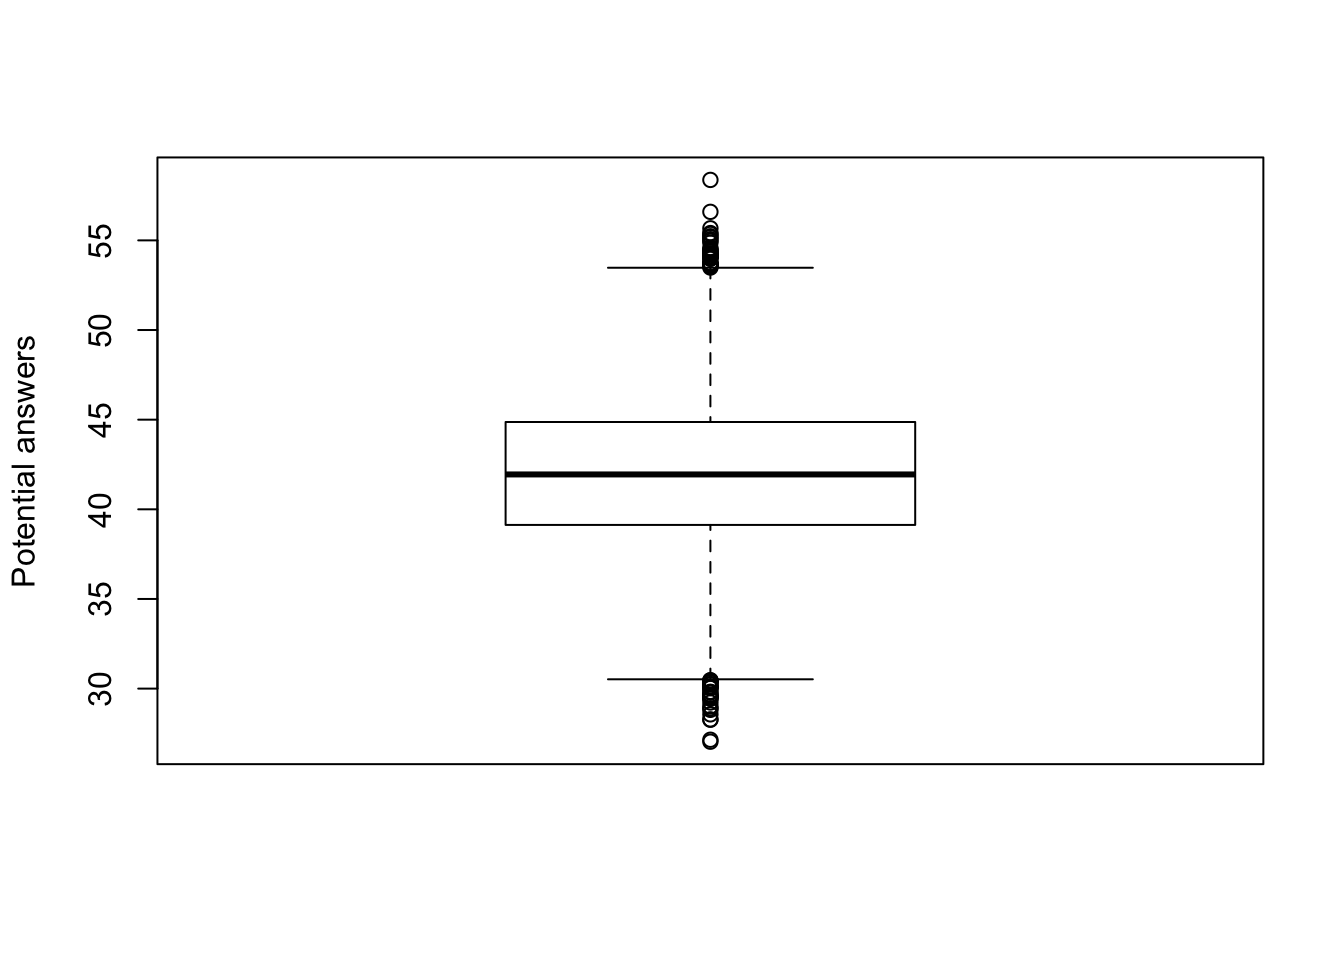
\includegraphics{bookdown-demo_files/figure-latex/unnamed-chunk-9-1} \end{center}

There are many other options we can include to customise our tree.

\begin{Shaded}
\begin{Highlighting}[]
\KeywordTok{ggtree}\NormalTok{(tree, }
       \DataTypeTok{branch.length=}\StringTok{"none"}\NormalTok{, }
       \DataTypeTok{color=}\StringTok{"blue"}\NormalTok{, }
       \DataTypeTok{size=}\DecValTok{2}\NormalTok{, }
       \DataTypeTok{linetype=}\DecValTok{3}\NormalTok{)}
\end{Highlighting}
\end{Shaded}

\begin{center}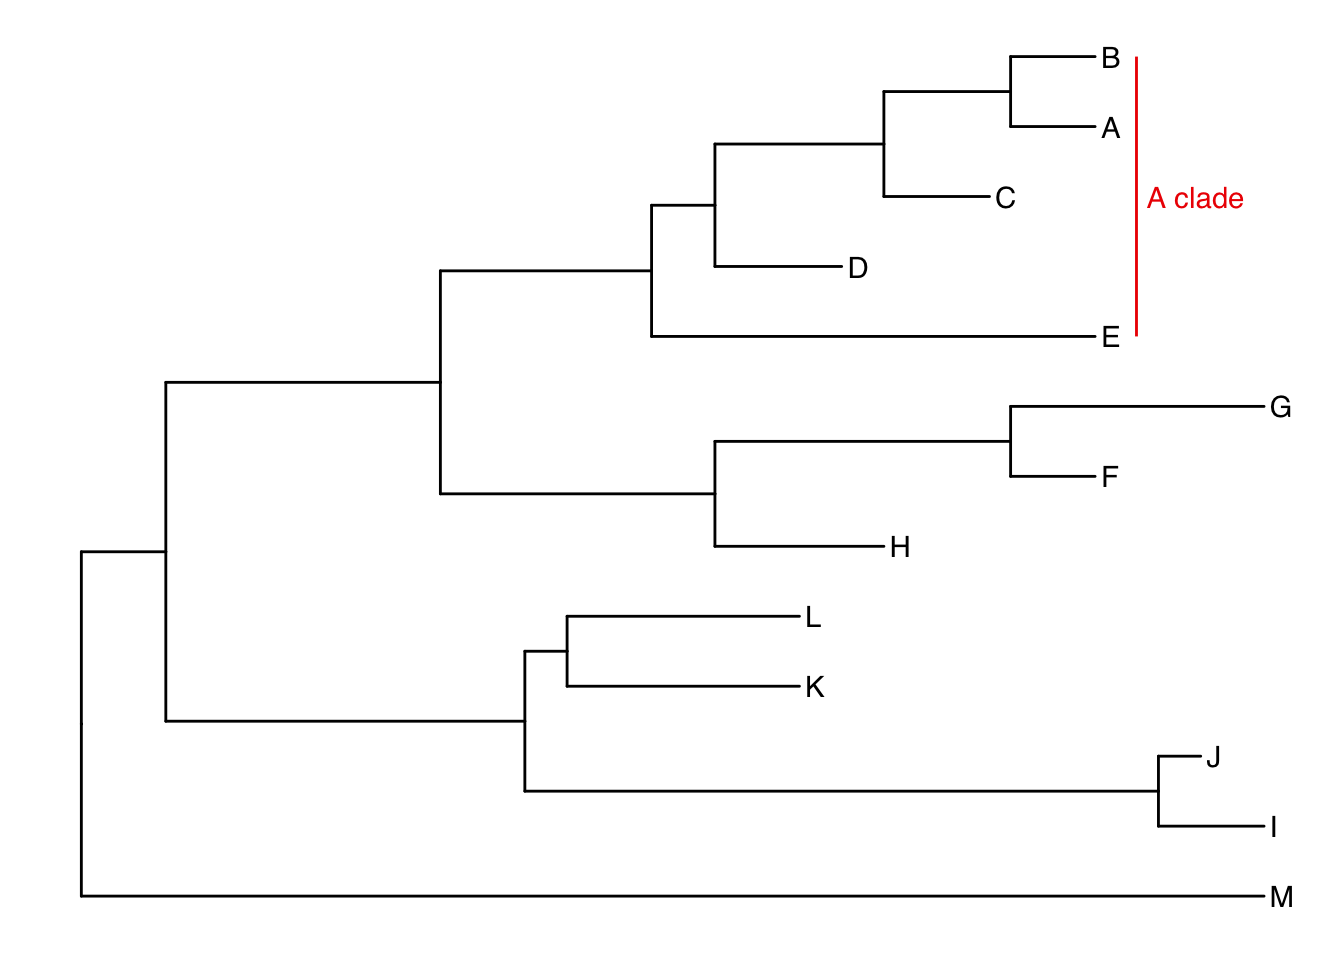
\includegraphics{bookdown-demo_files/figure-latex/unnamed-chunk-10-1} \end{center}

\subsection{Geoms}\label{geoms}

Geoms are new layers to plot on or alongside your tree. Here I'm
creating the plot as an object in R. You should see ``p'' appear in your
environment but no plot will appear.

\begin{Shaded}
\begin{Highlighting}[]
\NormalTok{p <-}\StringTok{ }\KeywordTok{ggtree}\NormalTok{(tree)}
\end{Highlighting}
\end{Shaded}

Now let's plot it whilst adding new layers. Note that the hash denotes
text not to be interpreted by R. This is a great way to annotate your
code so that you can recall what it does!

\begin{Shaded}
\begin{Highlighting}[]
\NormalTok{p }\OperatorTok{+}\StringTok{ }\KeywordTok{geom_nodepoint}\NormalTok{() }\CommentTok{#Add node points}
\end{Highlighting}
\end{Shaded}

\begin{center}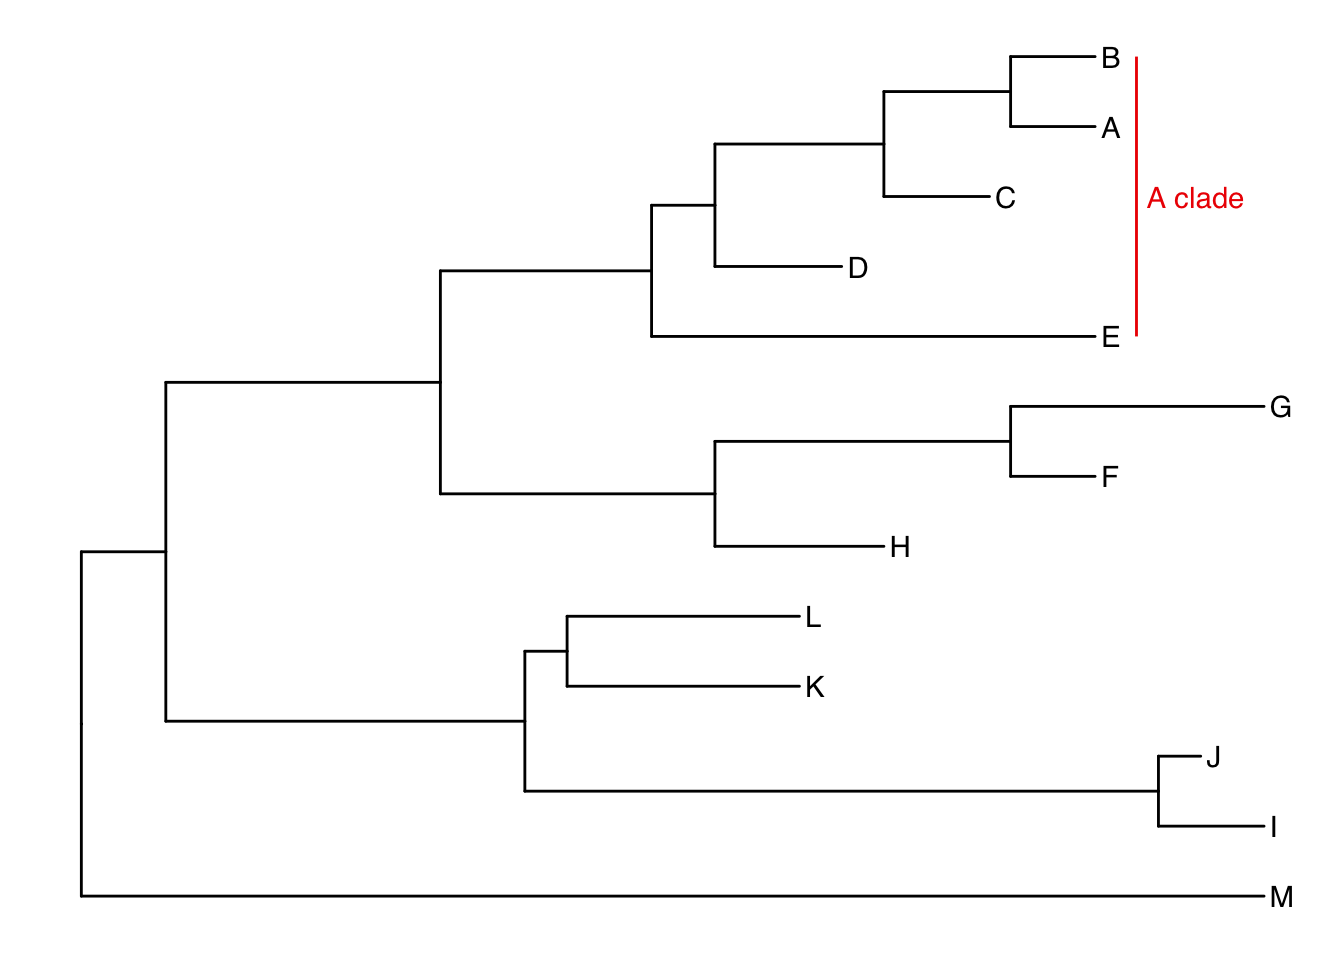
\includegraphics{bookdown-demo_files/figure-latex/unnamed-chunk-12-1} \end{center}

\begin{Shaded}
\begin{Highlighting}[]
\NormalTok{p }\OperatorTok{+}\StringTok{ }\KeywordTok{geom_tippoint}\NormalTok{() }\CommentTok{# add tip points}
\end{Highlighting}
\end{Shaded}

\begin{center}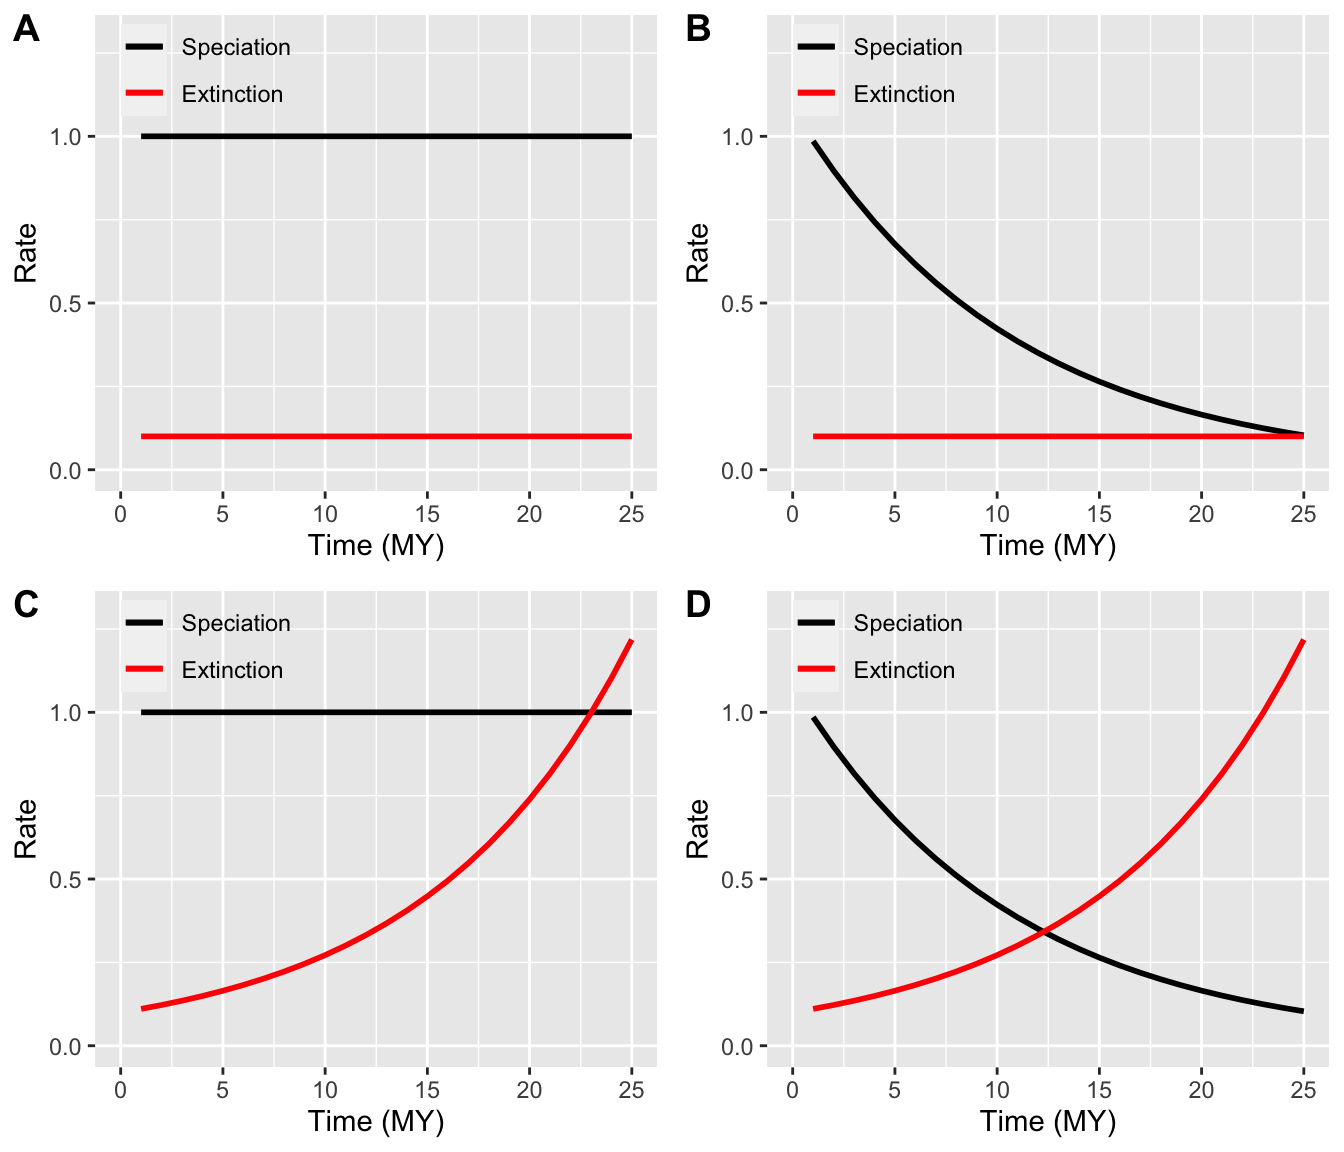
\includegraphics{bookdown-demo_files/figure-latex/unnamed-chunk-13-1} \end{center}

\begin{Shaded}
\begin{Highlighting}[]
\NormalTok{p }\OperatorTok{+}\StringTok{ }\KeywordTok{geom_tiplab}\NormalTok{() }\CommentTok{# Label the tips}
\end{Highlighting}
\end{Shaded}

\begin{center}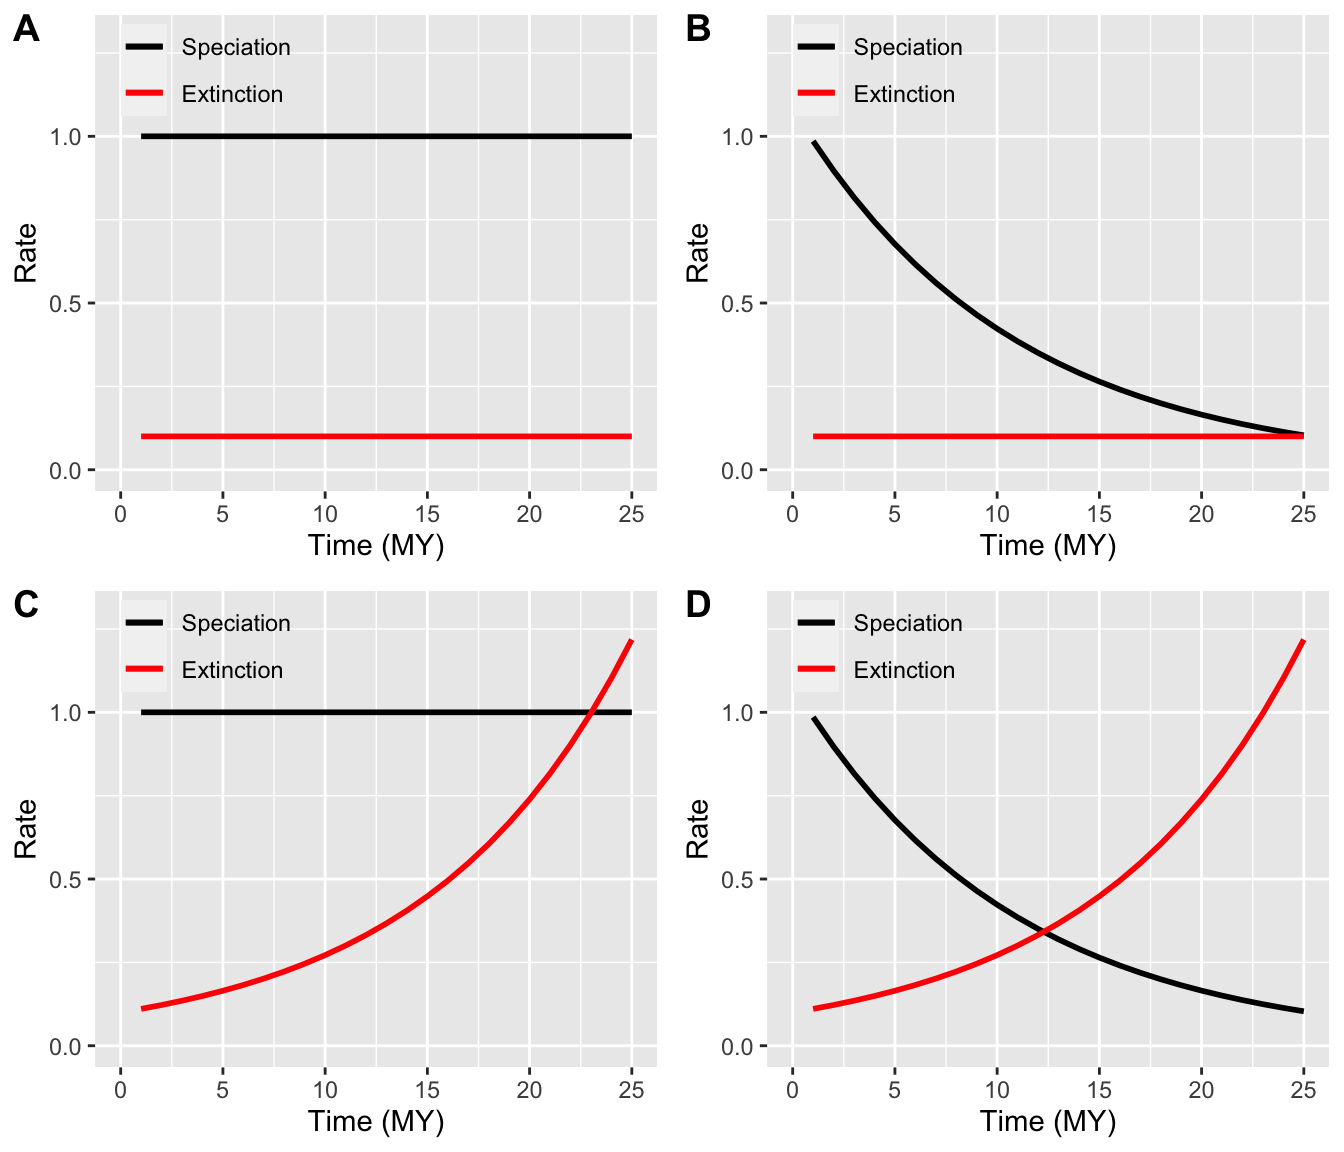
\includegraphics{bookdown-demo_files/figure-latex/unnamed-chunk-14-1} \end{center}

These geoms can be combined as you see fit. This gives you a lot of
flexibility in how you plot your trees.

\begin{Shaded}
\begin{Highlighting}[]
\NormalTok{p }\OperatorTok{+}\StringTok{ }
\StringTok{  }\KeywordTok{geom_tiplab}\NormalTok{(}\DataTypeTok{offset =} \DecValTok{2}\NormalTok{, }\DataTypeTok{color =} \StringTok{"purple"}\NormalTok{) }\OperatorTok{+}
\StringTok{  }\KeywordTok{geom_nodepoint}\NormalTok{(}\DataTypeTok{color =} \StringTok{"blue"}\NormalTok{, }\DataTypeTok{size =} \DecValTok{2}\NormalTok{) }\OperatorTok{+}
\StringTok{  }\KeywordTok{geom_tippoint}\NormalTok{(}\DataTypeTok{color =} \StringTok{"red"}\NormalTok{, }\DataTypeTok{size =} \DecValTok{4}\NormalTok{) }\OperatorTok{+}
\StringTok{  }\KeywordTok{ggtitle}\NormalTok{(}\StringTok{"A phylogeny of letters. For some reason..."}\NormalTok{)}
\end{Highlighting}
\end{Shaded}

\begin{center}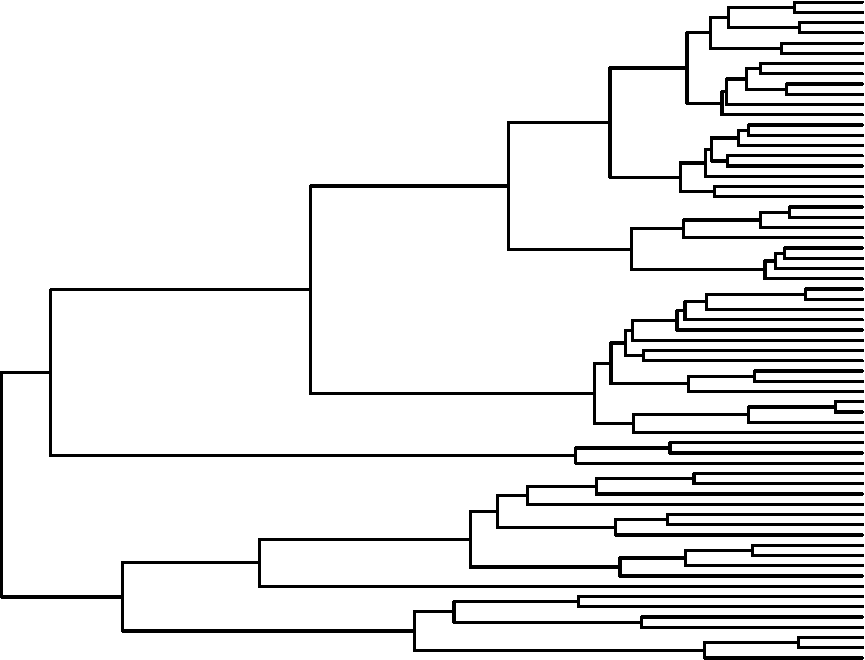
\includegraphics{bookdown-demo_files/figure-latex/unnamed-chunk-15-1} \end{center}

\subsection{Labelling clades}\label{labelling-clades}

To label clades, we need to be able to identify the node of the most
recent common ancestor. The function \textbf{MRCA} tells us that the
common ancestor of C and E is node 17.

\begin{Shaded}
\begin{Highlighting}[]
\KeywordTok{MRCA}\NormalTok{(tree, }\DataTypeTok{tip =} \KeywordTok{c}\NormalTok{(}\StringTok{"C"}\NormalTok{, }\StringTok{"E"}\NormalTok{))}
\end{Highlighting}
\end{Shaded}

\begin{verbatim}
[1] 17
\end{verbatim}

Let's use a new geom to label the clade.

\begin{Shaded}
\begin{Highlighting}[]
\KeywordTok{ggtree}\NormalTok{(tree) }\OperatorTok{+}\StringTok{ }
\StringTok{  }\KeywordTok{geom_tiplab}\NormalTok{() }\OperatorTok{+}\StringTok{ }
\StringTok{  }\KeywordTok{geom_cladelabel}\NormalTok{(}\DataTypeTok{node=}\DecValTok{17}\NormalTok{, }
                  \DataTypeTok{label=}\StringTok{"A clade"}\NormalTok{, }
                  \DataTypeTok{color=}\StringTok{"red2"}\NormalTok{, }
                  \DataTypeTok{offset=}\DecValTok{1}\NormalTok{)}
\end{Highlighting}
\end{Shaded}

\begin{center}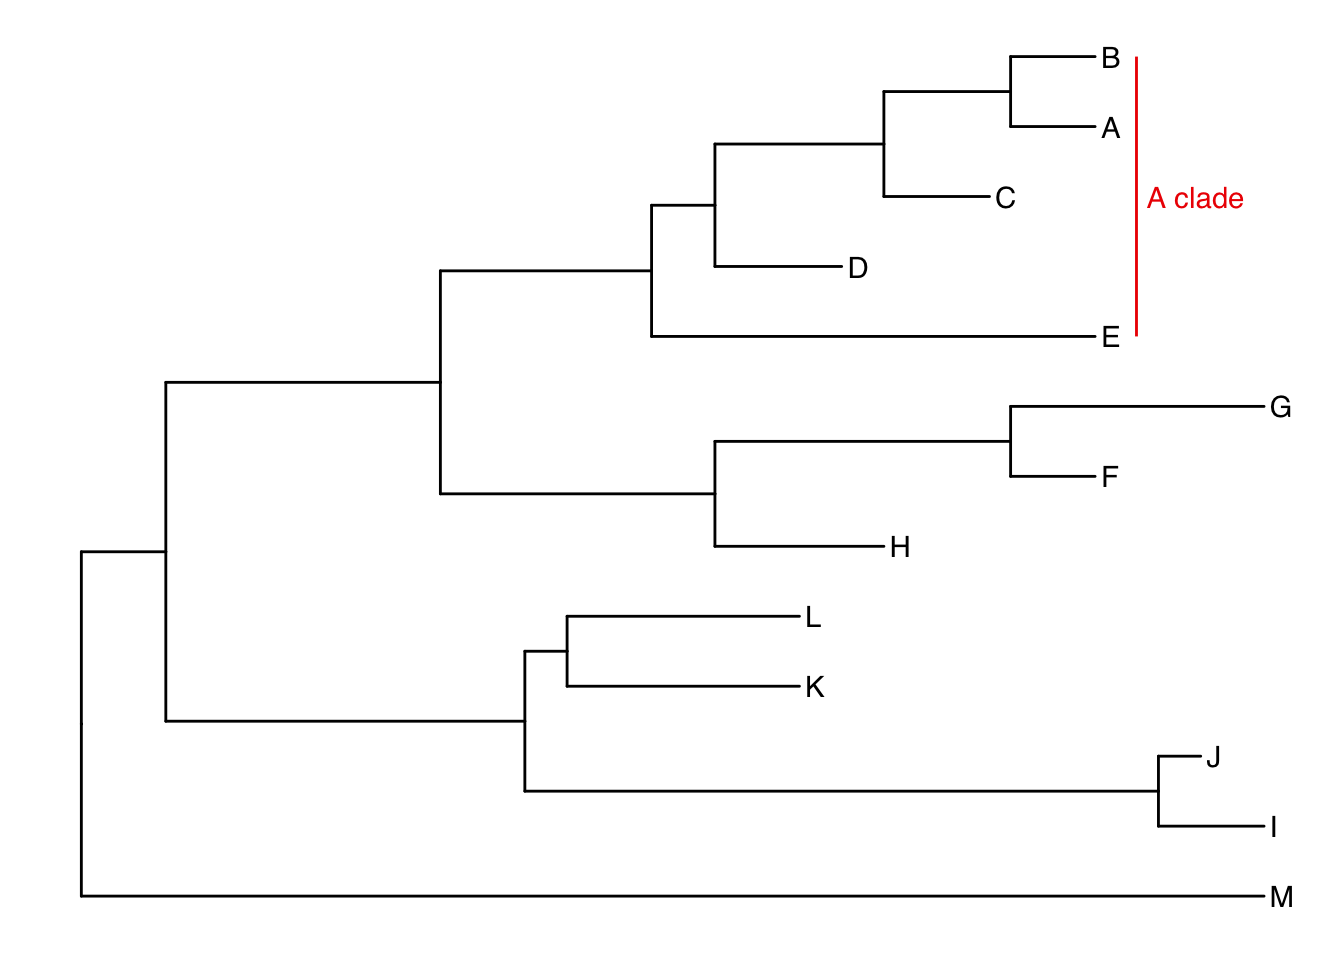
\includegraphics{bookdown-demo_files/figure-latex/unnamed-chunk-17-1} \end{center}

Pretty good. But there are other options. Again it's a matter of
personal preference. You may prefer to overlay a translucent rectangle
over your clade of interest.

\begin{Shaded}
\begin{Highlighting}[]
\KeywordTok{ggtree}\NormalTok{(tree) }\OperatorTok{+}\StringTok{ }
\StringTok{  }\KeywordTok{geom_tiplab}\NormalTok{() }\OperatorTok{+}\StringTok{ }
\StringTok{  }\KeywordTok{geom_hilight}\NormalTok{(}\DataTypeTok{node=}\DecValTok{17}\NormalTok{, }\DataTypeTok{fill=}\StringTok{"gold"}\NormalTok{)}
\end{Highlighting}
\end{Shaded}

\begin{center}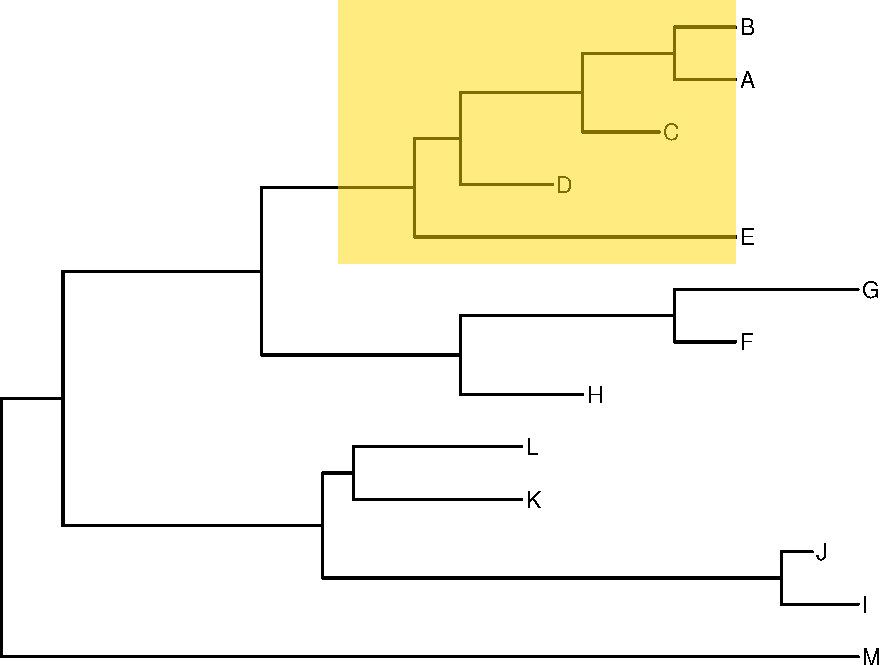
\includegraphics{bookdown-demo_files/figure-latex/unnamed-chunk-18-1} \end{center}

\section{Example Phylogeny}\label{example-phylogeny}

Let's now have a look at how we can include images on our plots. Using
images is a great way to annotate a phylogeny. Here's the kind of thing
I mean.

\begin{center}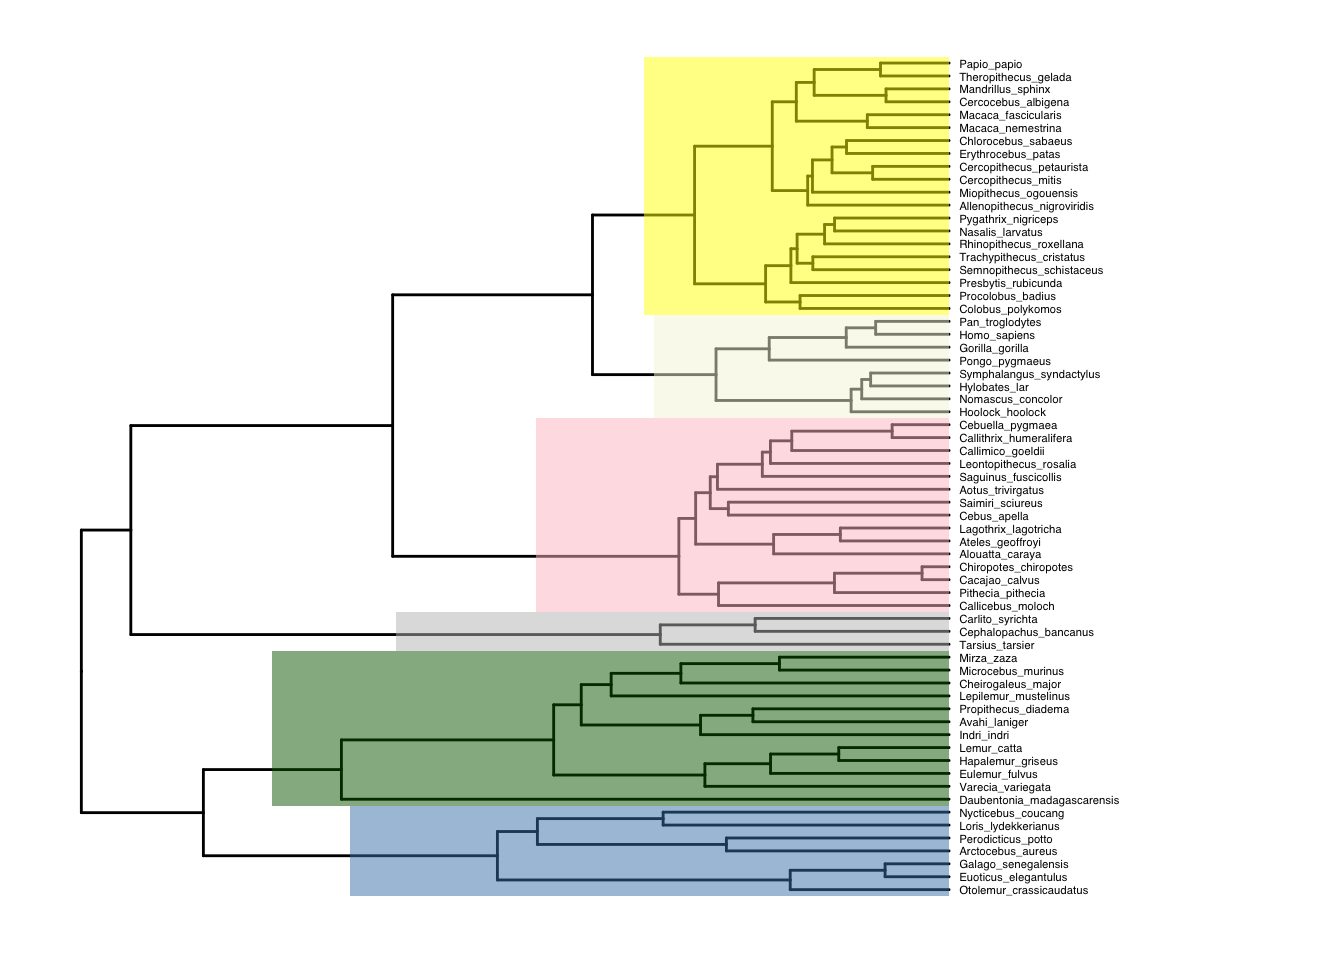
\includegraphics{bookdown-demo_files/figure-latex/unnamed-chunk-19-1} \end{center}

This phylogeny is annotated in a number of useful ways. The tip labels
are the most common type you probably recognise and in this case,
describe cephalopod families. The superorders (octopodiformes and
decapodiformes) are highlighted by gold and red rectangles as well as a
bar across the tips.

The most interesting thing for our purposes are the silhouettes at the
root of each superorder. The octopodiformes have an octopus and the
decapodiformes have a squid as example taxa from within the superorder.

\subsection{Phylopic}\label{phylopic}

The silhouettes I used for that plot are from a website
(\url{http://phylopic.org/}). Phylopic provides open source biological
silhouettes that are free to use. We're now going to look at how to do
this.

Let's start with loading an example tree. This one is a primate tree
courtesy of Randi Griffin. You'll notice that I'm loading this tree
using a url. This is because I'm loading a file directly from GitHub, a
sort of social network of coding and the host of this site! Randi (and
many other coders) make some of the things they produce freely available
through GitHub. This can be data, files or code.

\begin{Shaded}
\begin{Highlighting}[]
\NormalTok{primates <-}\StringTok{ }\KeywordTok{read.nexus}\NormalTok{(}\StringTok{"https://raw.githubusercontent.com/rgriff23/Dissertation/master/Chapter_2/data/tree.nex"}\NormalTok{)}
\end{Highlighting}
\end{Shaded}

Let's plot the new tree first.

\begin{Shaded}
\begin{Highlighting}[]
\NormalTok{p1 <-}\StringTok{ }\KeywordTok{ggtree}\NormalTok{(primates)}
\NormalTok{p1}
\end{Highlighting}
\end{Shaded}

\begin{center}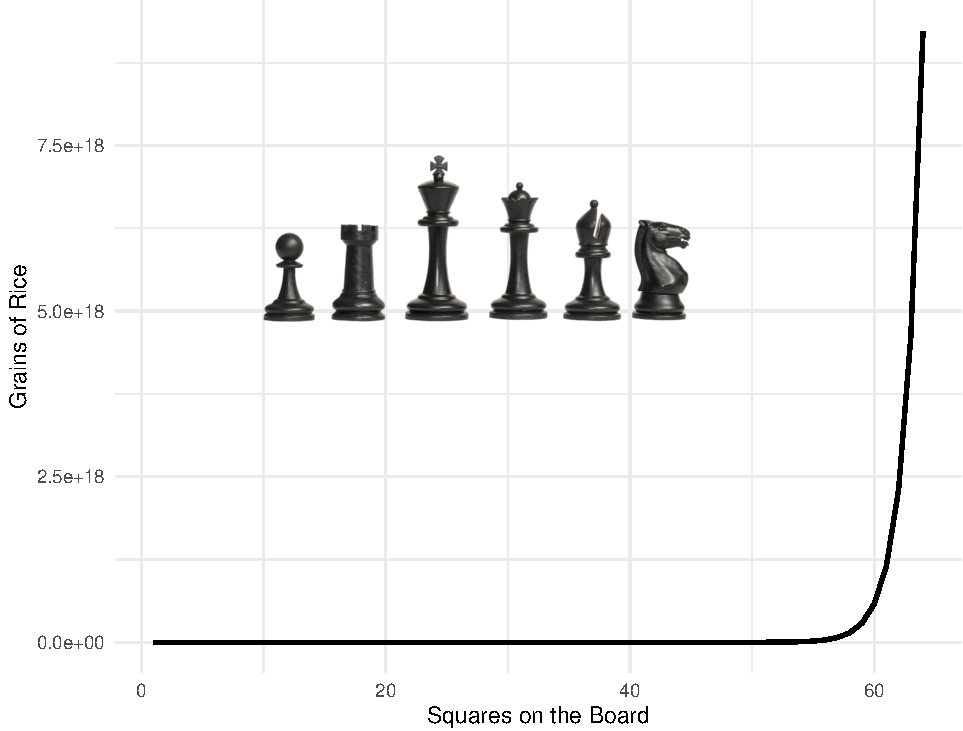
\includegraphics{bookdown-demo_files/figure-latex/unnamed-chunk-22-1} \end{center}

Let's use what we know about ggtree to customise this plot into
something more useful. In particular, this plot is quite useful because
it tells us the numbers of each node and we will need that later on.

\begin{Shaded}
\begin{Highlighting}[]
\NormalTok{p2 <-}\StringTok{ }\KeywordTok{ggtree}\NormalTok{(primates) }\OperatorTok{+}
\StringTok{  }\KeywordTok{xlim}\NormalTok{(}\DecValTok{0}\NormalTok{,}\DecValTok{90}\NormalTok{) }\OperatorTok{+}\StringTok{ }
\StringTok{  }\KeywordTok{geom_tiplab}\NormalTok{(}\DataTypeTok{size=}\FloatTok{1.5}\NormalTok{) }\OperatorTok{+}
\StringTok{  }\KeywordTok{geom_label2}\NormalTok{(}\KeywordTok{aes}\NormalTok{(}\DataTypeTok{subset=}\OperatorTok{!}\NormalTok{isTip, }\DataTypeTok{label=}\NormalTok{node), }\DataTypeTok{size=}\DecValTok{2}\NormalTok{, }\DataTypeTok{color=}\StringTok{"darkred"}\NormalTok{, }\DataTypeTok{alpha=}\FloatTok{0.5}\NormalTok{)}
\NormalTok{p2}
\end{Highlighting}
\end{Shaded}

\begin{center}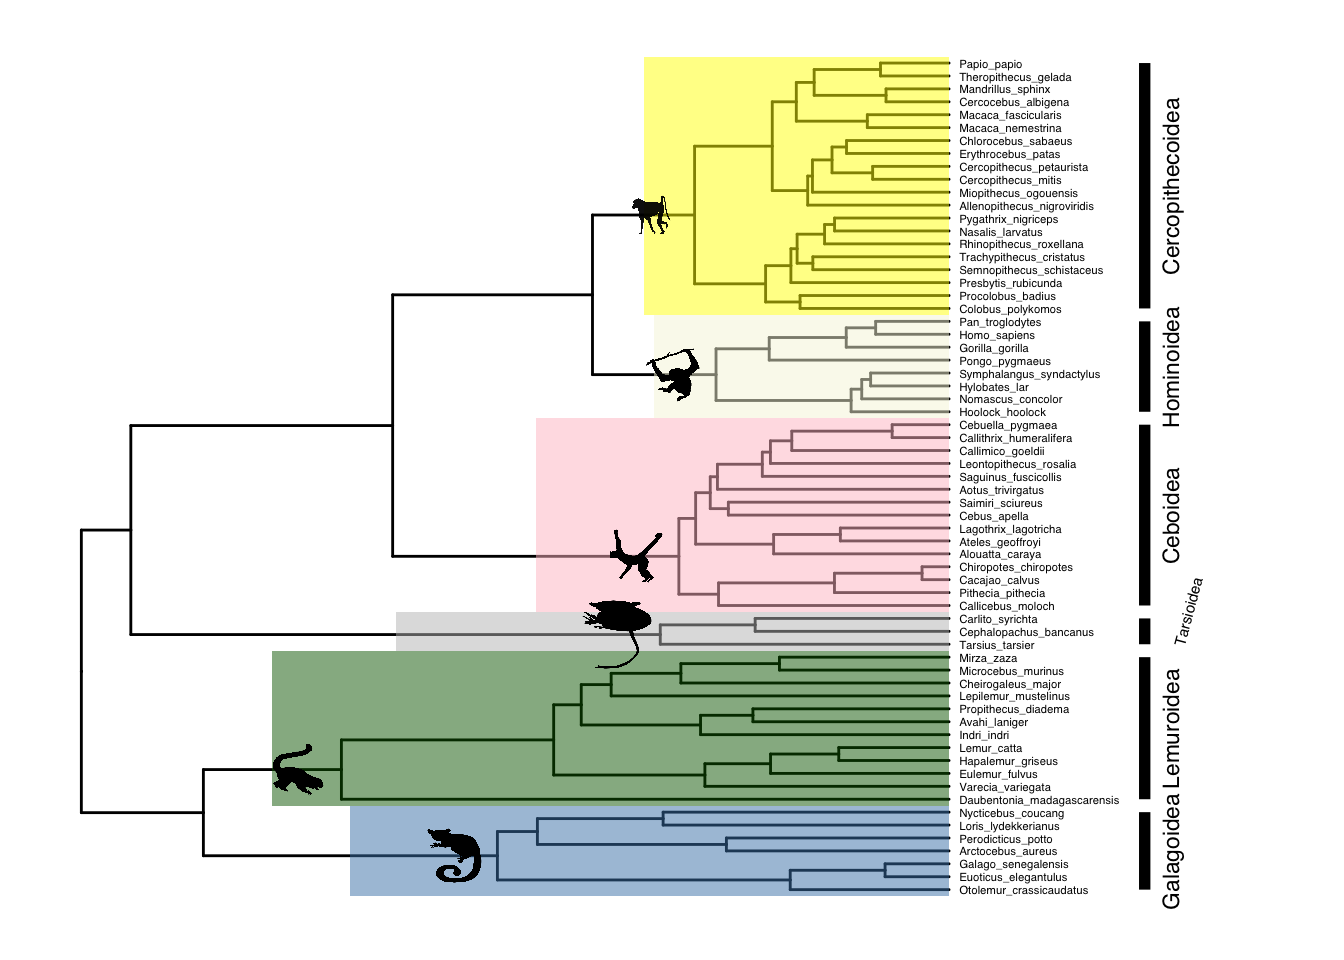
\includegraphics{bookdown-demo_files/figure-latex/unnamed-chunk-23-1} \end{center}

Let's label the 6 primate superfamilies.

\begin{Shaded}
\begin{Highlighting}[]
\NormalTok{p3 <-}\StringTok{ }\KeywordTok{ggtree}\NormalTok{(primates) }\OperatorTok{+}
\StringTok{  }\KeywordTok{xlim}\NormalTok{(}\DecValTok{0}\NormalTok{,}\DecValTok{100}\NormalTok{) }\OperatorTok{+}
\StringTok{  }\KeywordTok{geom_tiplab}\NormalTok{(}\DataTypeTok{size=}\FloatTok{1.5}\NormalTok{, }\DataTypeTok{offset=}\FloatTok{0.5}\NormalTok{) }\OperatorTok{+}
\StringTok{  }\KeywordTok{geom_hilight}\NormalTok{(}\DataTypeTok{node=}\DecValTok{124}\NormalTok{, }\DataTypeTok{fill=}\StringTok{"steelblue"}\NormalTok{, }\DataTypeTok{alpha=}\FloatTok{0.5}\NormalTok{) }\OperatorTok{+}
\StringTok{  }\KeywordTok{geom_hilight}\NormalTok{(}\DataTypeTok{node=}\DecValTok{113}\NormalTok{, }\DataTypeTok{fill=}\StringTok{"darkgreen"}\NormalTok{, }\DataTypeTok{alpha=}\FloatTok{0.5}\NormalTok{) }\OperatorTok{+}
\StringTok{  }\KeywordTok{geom_hilight}\NormalTok{(}\DataTypeTok{node=}\DecValTok{110}\NormalTok{, }\DataTypeTok{fill=}\StringTok{"gray"}\NormalTok{, }\DataTypeTok{alpha=}\FloatTok{0.5}\NormalTok{) }\OperatorTok{+}
\StringTok{  }\KeywordTok{geom_hilight}\NormalTok{(}\DataTypeTok{node=}\DecValTok{96}\NormalTok{, }\DataTypeTok{fill=}\StringTok{"pink"}\NormalTok{, }\DataTypeTok{alpha=}\FloatTok{0.5}\NormalTok{) }\OperatorTok{+}
\StringTok{  }\KeywordTok{geom_hilight}\NormalTok{(}\DataTypeTok{node=}\DecValTok{89}\NormalTok{, }\DataTypeTok{fill=}\StringTok{"beige"}\NormalTok{, }\DataTypeTok{alpha=}\FloatTok{0.5}\NormalTok{) }\OperatorTok{+}
\StringTok{  }\KeywordTok{geom_hilight}\NormalTok{(}\DataTypeTok{node=}\DecValTok{70}\NormalTok{, }\DataTypeTok{fill=}\StringTok{"yellow"}\NormalTok{, }\DataTypeTok{alpha=}\FloatTok{0.5}\NormalTok{) }
\NormalTok{p3}
\end{Highlighting}
\end{Shaded}

\begin{center}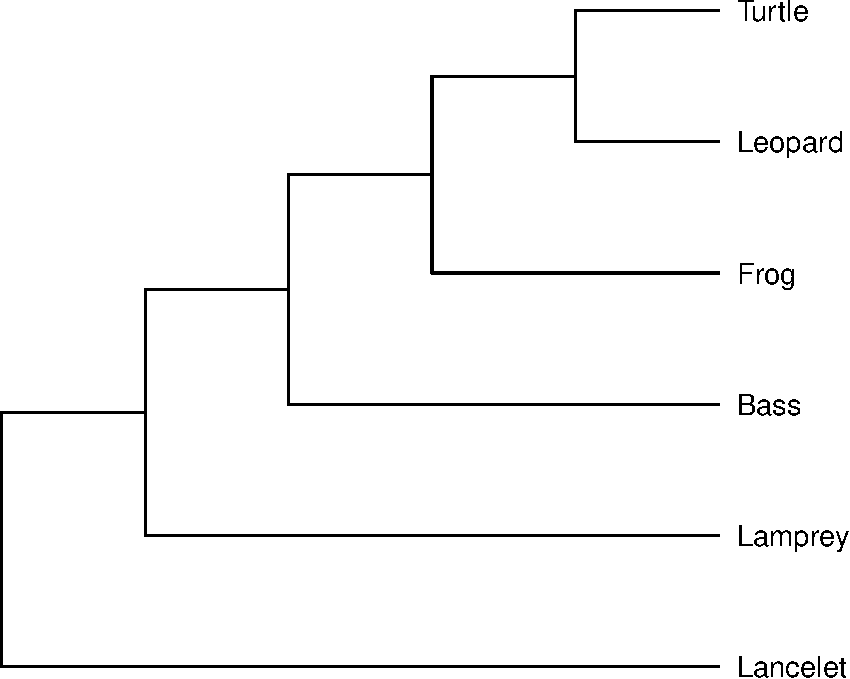
\includegraphics{bookdown-demo_files/figure-latex/unnamed-chunk-24-1} \end{center}

So far so good. Let's add on bars like I did for the cephalopod version.
This time, I'll add the new details to the object p3 to save some
typing.

\begin{Shaded}
\begin{Highlighting}[]
\NormalTok{p4 <-}\StringTok{ }\NormalTok{p3 }\OperatorTok{+}
\StringTok{  }\KeywordTok{geom_cladelabel}\NormalTok{(}\DecValTok{124}\NormalTok{, }\StringTok{"Galagoidea"}\NormalTok{, }\DataTypeTok{offset=}\DecValTok{15}\NormalTok{, }\DataTypeTok{barsize=}\DecValTok{2}\NormalTok{, }\DataTypeTok{angle=}\DecValTok{90}\NormalTok{,}
                  \DataTypeTok{offset.text=}\FloatTok{1.5}\NormalTok{, }\DataTypeTok{hjust=}\FloatTok{0.5}\NormalTok{, }\DataTypeTok{fontsize=}\DecValTok{3}\NormalTok{) }\OperatorTok{+}\StringTok{ }
\StringTok{  }\KeywordTok{geom_cladelabel}\NormalTok{(}\DecValTok{113}\NormalTok{, }\StringTok{"Lemuroidea"}\NormalTok{, }\DataTypeTok{offset=}\DecValTok{15}\NormalTok{, }\DataTypeTok{barsize=}\DecValTok{2}\NormalTok{, }\DataTypeTok{angle=}\DecValTok{90}\NormalTok{,}
                  \DataTypeTok{offset.text=}\FloatTok{1.5}\NormalTok{, }\DataTypeTok{hjust=}\FloatTok{0.5}\NormalTok{, }\DataTypeTok{fontsize=}\DecValTok{3}\NormalTok{) }\OperatorTok{+}
\StringTok{  }\KeywordTok{geom_cladelabel}\NormalTok{(}\DecValTok{110}\NormalTok{, }\StringTok{"Tarsioidea"}\NormalTok{, }\DataTypeTok{offset=}\DecValTok{15}\NormalTok{, }\DataTypeTok{barsize=}\DecValTok{2}\NormalTok{, }\DataTypeTok{angle=}\DecValTok{75}\NormalTok{,}
                  \DataTypeTok{offset.text=}\FloatTok{2.5}\NormalTok{, }\DataTypeTok{hjust=}\FloatTok{0.2}\NormalTok{, }\DataTypeTok{fontsize=}\DecValTok{2}\NormalTok{) }\OperatorTok{+}
\StringTok{  }\KeywordTok{geom_cladelabel}\NormalTok{(}\DecValTok{96}\NormalTok{, }\StringTok{"Ceboidea"}\NormalTok{, }\DataTypeTok{offset=}\DecValTok{15}\NormalTok{, }\DataTypeTok{barsize=}\DecValTok{2}\NormalTok{, }\DataTypeTok{angle=}\DecValTok{90}\NormalTok{,}
                  \DataTypeTok{offset.text=}\FloatTok{1.5}\NormalTok{, }\DataTypeTok{hjust=}\FloatTok{0.5}\NormalTok{, }\DataTypeTok{fontsize=}\DecValTok{3}\NormalTok{) }\OperatorTok{+}
\StringTok{  }\KeywordTok{geom_cladelabel}\NormalTok{(}\DecValTok{89}\NormalTok{, }\StringTok{"Hominoidea"}\NormalTok{, }\DataTypeTok{offset=}\DecValTok{15}\NormalTok{, }\DataTypeTok{barsize=}\DecValTok{2}\NormalTok{, }\DataTypeTok{angle=}\DecValTok{90}\NormalTok{,}
                  \DataTypeTok{offset.text=}\FloatTok{1.5}\NormalTok{, }\DataTypeTok{hjust=}\FloatTok{0.5}\NormalTok{, }\DataTypeTok{fontsize=}\DecValTok{3}\NormalTok{) }\OperatorTok{+}
\StringTok{  }\KeywordTok{geom_cladelabel}\NormalTok{(}\DecValTok{70}\NormalTok{, }\StringTok{"Cercopithecoidea"}\NormalTok{, }\DataTypeTok{offset=}\DecValTok{15}\NormalTok{, }\DataTypeTok{barsize=}\DecValTok{2}\NormalTok{, }\DataTypeTok{angle=}\DecValTok{90}\NormalTok{,}
                  \DataTypeTok{offset.text=}\FloatTok{1.5}\NormalTok{, }\DataTypeTok{hjust=}\FloatTok{0.5}\NormalTok{, }\DataTypeTok{fontsize=}\DecValTok{3}\NormalTok{)}
\NormalTok{p4}
\end{Highlighting}
\end{Shaded}

\begin{center}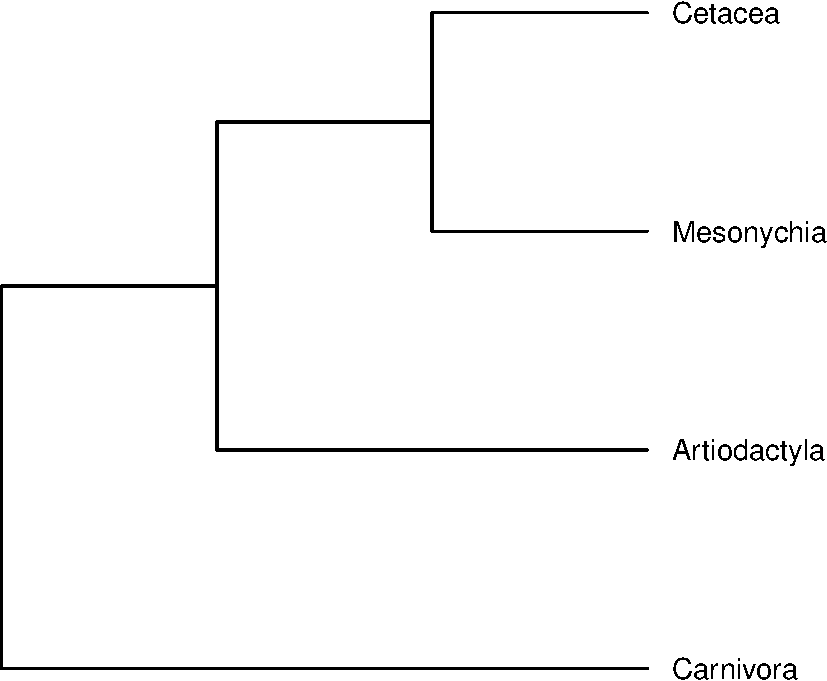
\includegraphics{bookdown-demo_files/figure-latex/unnamed-chunk-25-1} \end{center}

There are some helpful details here, such as the fact that the label for
Tarsioidea is off at an angle to avoid overlapping with other labels.
The extra arguments in these options demonstrate how much control you
can exercise over each geom.

Now let's get to adding images. the way to do this is a little awkward
with ggtree but I think it's worth the hassle. The first thing we have
to do is gather the links for each image we want to use. I've chosen to
do this by building a small data frame containing the urls to the images
on phylopic, the names of the super families I want to label and the
nodes I want to plot the images on.

\begin{Shaded}
\begin{Highlighting}[]
\NormalTok{images <-}\StringTok{ }\KeywordTok{data.frame}\NormalTok{(}\DataTypeTok{node =} \KeywordTok{c}\NormalTok{(}\DecValTok{124}\NormalTok{,}\DecValTok{113}\NormalTok{,}\DecValTok{110}\NormalTok{,}\DecValTok{96}\NormalTok{,}\DecValTok{89}\NormalTok{,}\DecValTok{70}\NormalTok{),}
                     \DataTypeTok{phylopic =} \KeywordTok{c}\NormalTok{(}\StringTok{"http://phylopic.org/assets/images/submissions/}
\StringTok{                                  7fb9bea8-e758-4986-afb2-95a2c3bf983d.512.png"}\NormalTok{,}
                                  \StringTok{"http://phylopic.org/assets/images/submissions/}
\StringTok{                                  bac25f49-97a4-4aec-beb6-f542158ebd23.512.png"}\NormalTok{,}
                                  \StringTok{"http://phylopic.org/assets/images/submissions/}
\StringTok{                                  f598fb39-facf-43ea-a576-1861304b2fe4.512.png"}\NormalTok{,}
                                  \StringTok{"http://phylopic.org/assets/images/submissions/}
\StringTok{                                  aceb287d-84cf-46f1-868c-4797c4ac54a8.512.png"}\NormalTok{,}
                                  \StringTok{"http://phylopic.org/assets/images/submissions/}
\StringTok{                                  0174801d-15a6-4668-bfe0-4c421fbe51e8.512.png"}\NormalTok{,}
                                  \StringTok{"http://phylopic.org/assets/images/submissions/}
\StringTok{                                  72f2f854-f3cd-4666-887c-35d5c256ab0f.512.png"}\NormalTok{),}
                     \DataTypeTok{species =} \KeywordTok{c}\NormalTok{(}\StringTok{"Galagoidea"}\NormalTok{,}\StringTok{"Lemuroidea"}\NormalTok{,}\StringTok{"Tarsioidea"}\NormalTok{,}
                                 \StringTok{"Ceboidea"}\NormalTok{,}\StringTok{"Hominoidea"}\NormalTok{,}\StringTok{"Cercopithecoidea"}\NormalTok{))}
\end{Highlighting}
\end{Shaded}

This is a way of plotting them all at once with all the code included to
build the plot from scratch.

\begin{Shaded}
\begin{Highlighting}[]
\NormalTok{p5 <-}\StringTok{ }\KeywordTok{ggtree}\NormalTok{(primates) }\OperatorTok{+}
\StringTok{  }\KeywordTok{xlim}\NormalTok{(}\DecValTok{0}\NormalTok{,}\DecValTok{110}\NormalTok{) }\OperatorTok{+}
\StringTok{  }\KeywordTok{geom_tiplab}\NormalTok{(}\DataTypeTok{size=}\DecValTok{2}\NormalTok{, }\DataTypeTok{offset=}\FloatTok{0.5}\NormalTok{) }\OperatorTok{+}
\StringTok{  }\KeywordTok{geom_hilight}\NormalTok{(}\DataTypeTok{node=}\DecValTok{124}\NormalTok{, }\DataTypeTok{fill=}\StringTok{"steelblue"}\NormalTok{, }\DataTypeTok{alpha=}\FloatTok{0.5}\NormalTok{) }\OperatorTok{+}
\StringTok{  }\KeywordTok{geom_hilight}\NormalTok{(}\DataTypeTok{node=}\DecValTok{113}\NormalTok{, }\DataTypeTok{fill=}\StringTok{"darkgreen"}\NormalTok{, }\DataTypeTok{alpha=}\FloatTok{0.5}\NormalTok{) }\OperatorTok{+}
\StringTok{  }\KeywordTok{geom_hilight}\NormalTok{(}\DataTypeTok{node=}\DecValTok{110}\NormalTok{, }\DataTypeTok{fill=}\StringTok{"gray"}\NormalTok{, }\DataTypeTok{alpha=}\FloatTok{0.5}\NormalTok{) }\OperatorTok{+}
\StringTok{  }\KeywordTok{geom_hilight}\NormalTok{(}\DataTypeTok{node=}\DecValTok{96}\NormalTok{, }\DataTypeTok{fill=}\StringTok{"pink"}\NormalTok{, }\DataTypeTok{alpha=}\FloatTok{0.5}\NormalTok{) }\OperatorTok{+}
\StringTok{  }\KeywordTok{geom_hilight}\NormalTok{(}\DataTypeTok{node=}\DecValTok{89}\NormalTok{, }\DataTypeTok{fill=}\StringTok{"beige"}\NormalTok{, }\DataTypeTok{alpha=}\FloatTok{0.5}\NormalTok{) }\OperatorTok{+}
\StringTok{  }\KeywordTok{geom_hilight}\NormalTok{(}\DataTypeTok{node=}\DecValTok{70}\NormalTok{, }\DataTypeTok{fill=}\StringTok{"yellow"}\NormalTok{, }\DataTypeTok{alpha=}\FloatTok{0.5}\NormalTok{) }\OperatorTok{+}
\StringTok{  }\KeywordTok{geom_cladelabel}\NormalTok{(}\DecValTok{124}\NormalTok{, }\StringTok{"Galagoidea"}\NormalTok{, }\DataTypeTok{offset=}\DecValTok{22}\NormalTok{, }\DataTypeTok{barsize=}\DecValTok{2}\NormalTok{, }\DataTypeTok{angle=}\DecValTok{90}\NormalTok{,}
                  \DataTypeTok{offset.text=}\FloatTok{1.5}\NormalTok{, }\DataTypeTok{hjust=}\FloatTok{0.5}\NormalTok{, }\DataTypeTok{fontsize=}\DecValTok{5}\NormalTok{) }\OperatorTok{+}\StringTok{ }
\StringTok{  }\KeywordTok{geom_cladelabel}\NormalTok{(}\DecValTok{113}\NormalTok{, }\StringTok{"Lemuroidea"}\NormalTok{, }\DataTypeTok{offset=}\DecValTok{22}\NormalTok{, }\DataTypeTok{barsize=}\DecValTok{2}\NormalTok{, }\DataTypeTok{angle=}\DecValTok{90}\NormalTok{,}
                  \DataTypeTok{offset.text=}\FloatTok{1.5}\NormalTok{, }\DataTypeTok{hjust=}\FloatTok{0.5}\NormalTok{, }\DataTypeTok{fontsize=}\DecValTok{5}\NormalTok{) }\OperatorTok{+}
\StringTok{  }\KeywordTok{geom_cladelabel}\NormalTok{(}\DecValTok{110}\NormalTok{, }\StringTok{"Tarsioidea"}\NormalTok{, }\DataTypeTok{offset=}\DecValTok{22}\NormalTok{, }\DataTypeTok{barsize=}\DecValTok{2}\NormalTok{, }\DataTypeTok{angle=}\DecValTok{75}\NormalTok{,}
                  \DataTypeTok{offset.text=}\FloatTok{2.5}\NormalTok{, }\DataTypeTok{hjust=}\FloatTok{0.2}\NormalTok{, }\DataTypeTok{fontsize=}\DecValTok{4}\NormalTok{) }\OperatorTok{+}
\StringTok{  }\KeywordTok{geom_cladelabel}\NormalTok{(}\DecValTok{96}\NormalTok{, }\StringTok{"Ceboidea"}\NormalTok{, }\DataTypeTok{offset=}\DecValTok{22}\NormalTok{, }\DataTypeTok{barsize=}\DecValTok{2}\NormalTok{, }\DataTypeTok{angle=}\DecValTok{90}\NormalTok{,}
                  \DataTypeTok{offset.text=}\FloatTok{1.5}\NormalTok{, }\DataTypeTok{hjust=}\FloatTok{0.5}\NormalTok{, }\DataTypeTok{fontsize=}\DecValTok{5}\NormalTok{) }\OperatorTok{+}
\StringTok{  }\KeywordTok{geom_cladelabel}\NormalTok{(}\DecValTok{89}\NormalTok{, }\StringTok{"Hominoidea"}\NormalTok{, }\DataTypeTok{offset=}\DecValTok{22}\NormalTok{, }\DataTypeTok{barsize=}\DecValTok{2}\NormalTok{, }\DataTypeTok{angle=}\DecValTok{90}\NormalTok{,}
                  \DataTypeTok{offset.text=}\FloatTok{1.5}\NormalTok{, }\DataTypeTok{hjust=}\FloatTok{0.5}\NormalTok{, }\DataTypeTok{fontsize=}\DecValTok{5}\NormalTok{) }\OperatorTok{+}
\StringTok{  }\KeywordTok{geom_cladelabel}\NormalTok{(}\DecValTok{70}\NormalTok{, }\StringTok{"Cercopithecoidea"}\NormalTok{, }\DataTypeTok{offset=}\DecValTok{22}\NormalTok{, }\DataTypeTok{barsize=}\DecValTok{2}\NormalTok{, }\DataTypeTok{angle=}\DecValTok{90}\NormalTok{,}
                  \DataTypeTok{offset.text=}\FloatTok{1.5}\NormalTok{, }\DataTypeTok{hjust=}\FloatTok{0.5}\NormalTok{, }\DataTypeTok{fontsize=}\DecValTok{5}\NormalTok{)}

\NormalTok{p5 }\OperatorTok\StringTok{ }\NormalTok{images }\OperatorTok{+}
\StringTok{  }\KeywordTok{geom_nodelab}\NormalTok{(}\KeywordTok{aes}\NormalTok{(}\DataTypeTok{image =}\NormalTok{ phylopic), }\DataTypeTok{geom =} \StringTok{"image"}\NormalTok{, }
               \DataTypeTok{size =}\NormalTok{ .}\DecValTok{04}\NormalTok{, }\DataTypeTok{nudge_x =} \OperatorTok{-}\DecValTok{4}\NormalTok{)}
\end{Highlighting}
\end{Shaded}

\begin{center}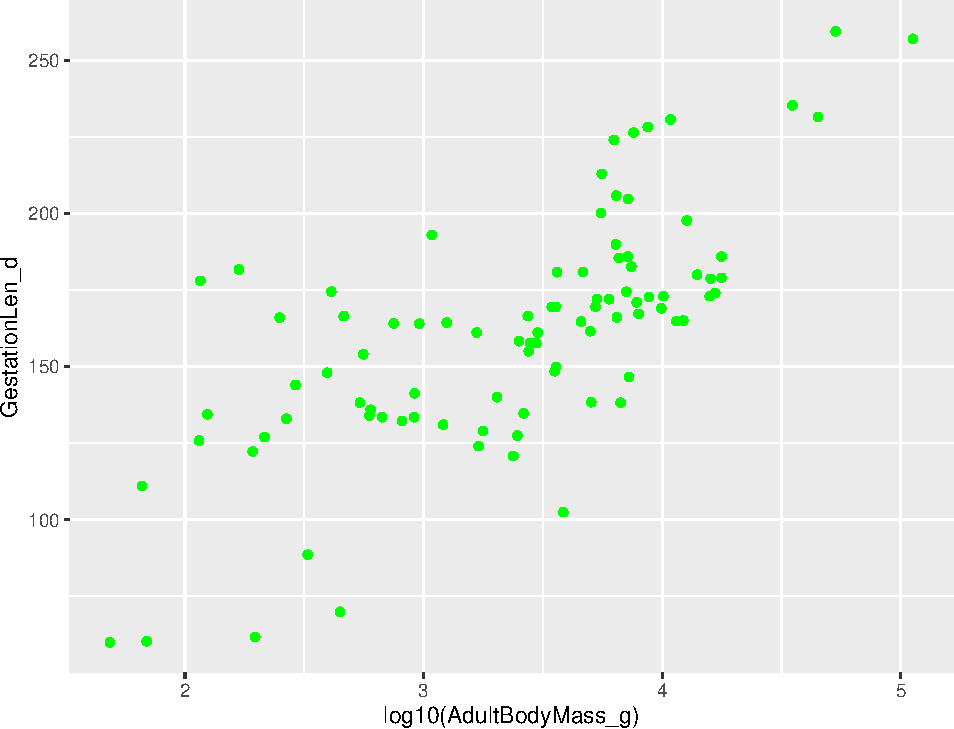
\includegraphics{bookdown-demo_files/figure-latex/unnamed-chunk-28-1} \end{center}

\chapter{Workshop 2: PGLS}\label{w2PGLS}

This tutorial will show you how to perform phylogenetically correct
regression analyses on continuous data in R.

As usual, remember to set your working directory to wherever you have
saved the necessary files. Other than that, this tutorial assumes you
have already installed the packages ape and caper.

\section{Data}\label{data}

Let's load up some primate data. You should see the dataframe appear in
your environment. If you inspect the object, you will find a number of
continuous variables in there for us to investigate.

\begin{Shaded}
\begin{Highlighting}[]
\NormalTok{primate.data <-}\StringTok{ }\KeywordTok{read.table}\NormalTok{(}\StringTok{"primates_data.txt"}\NormalTok{, }\DataTypeTok{header =}\NormalTok{ T)}
\KeywordTok{names}\NormalTok{(primate.data)}
\end{Highlighting}
\end{Shaded}

\begin{verbatim}
[1] "Order"           "Family"          "Binomial"        "AdultBodyMass_g"
[5] "GestationLen_d"  "HomeRange_km2"   "MaxLongevity_m"  "SocialGroupSize"
\end{verbatim}

\section{Plotting with ggplot2}\label{plotting-with-ggplot2}

A nice way of investigating data is by plotting it. For a quick
visualisation I usually use the base graphics in R. They get the job
done and are realtively simple to edit once you understand the syntax of
R.

However, most R users seem to agree that the package ``ggplot2'' gives
better plots. This might be useful to you when you want to prepare your
plots for reports. So here, I'm going to use ggplot2 just to show you
what it can do.

\begin{Shaded}
\begin{Highlighting}[]
\KeywordTok{install.packages}\NormalTok{(}\StringTok{"ggplot2"}\NormalTok{)}
\KeywordTok{library}\NormalTok{(ggplot2)}
\end{Highlighting}
\end{Shaded}

ggplot2 builds plots in layers similar to ggtree which you have met
before in workshop 1. In fact, the ggtree package was built based upon
ggplot2. We start with the function ggplot which creates a coordinate
system to which we can add layers. This function alone just creates a
blank plot

\begin{Shaded}
\begin{Highlighting}[]
\KeywordTok{ggplot}\NormalTok{(}\DataTypeTok{data =}\NormalTok{ primate.data)}
\end{Highlighting}
\end{Shaded}

\begin{center}
\includegraphics{bookdown-demo_files/figure-latex/unnamed-chunk-32-1} \end{center}

Let's add a layer with the points. We can add a layer of points with the
function geom\_point. This creates our basic scatterplot. Each geom
function (the ones that add layers) takes a mapping argument which
controls how the layer is mapped onto the plot. This argument usually
takes the form seen below. Remember that body mass should be log
transformed before we plot it!

\begin{Shaded}
\begin{Highlighting}[]
\KeywordTok{ggplot}\NormalTok{(}\DataTypeTok{data =}\NormalTok{ primate.data) }\OperatorTok{+}
\StringTok{  }\KeywordTok{geom_point}\NormalTok{(}\DataTypeTok{mapping =} \KeywordTok{aes}\NormalTok{(}\DataTypeTok{x =} \KeywordTok{log10}\NormalTok{(AdultBodyMass_g), }\DataTypeTok{y =}\NormalTok{ GestationLen_d))}
\end{Highlighting}
\end{Shaded}

\begin{center}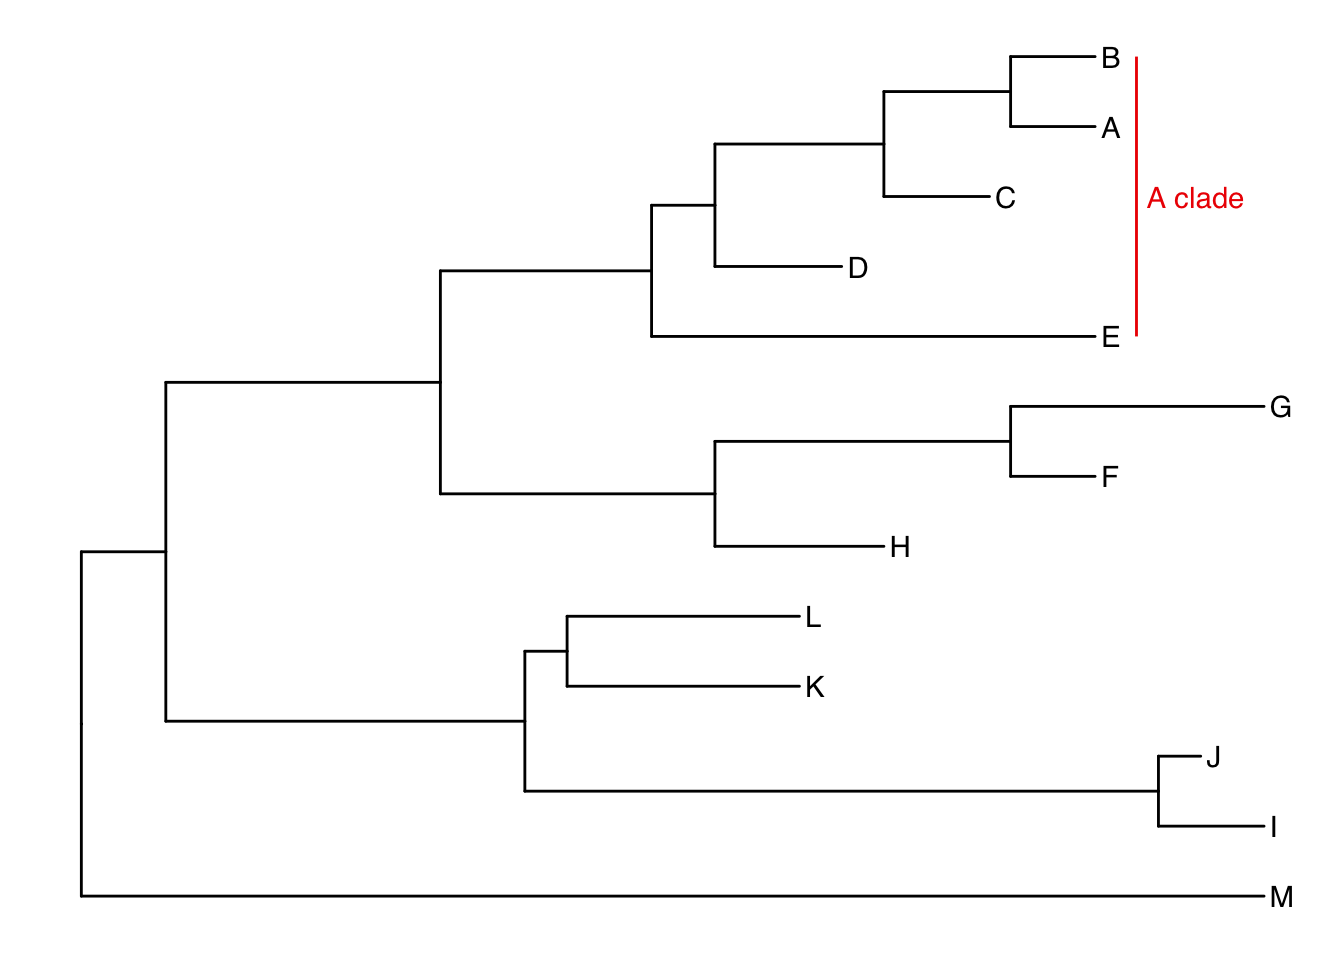
\includegraphics{bookdown-demo_files/figure-latex/unnamed-chunk-33-1} \end{center}

In practice, exactly how you add geoms and layers seems to be affected
by exactly what you want to do with the plot. As we'll see later, if you
want to add regression lines or other statistical features to your plot,
you may want to reorganise this code. My advice is to google what you
want to do and work backwards from someone else's code. That's what I
do.

The plot isn't done yet. We can display a bit more information by adding
another mapping argument. Here, I've coloured the points according to
their family. The unique colours are assigned auotmatically and the
legend is also created automatically.

\begin{Shaded}
\begin{Highlighting}[]
\KeywordTok{ggplot}\NormalTok{(}\DataTypeTok{data =}\NormalTok{ primate.data) }\OperatorTok{+}
\StringTok{  }\KeywordTok{geom_point}\NormalTok{(}\DataTypeTok{mapping =} \KeywordTok{aes}\NormalTok{(}\DataTypeTok{x =} \KeywordTok{log10}\NormalTok{(AdultBodyMass_g), }\DataTypeTok{y =}\NormalTok{ GestationLen_d, }
                           \DataTypeTok{colour =}\NormalTok{ Family))}
\end{Highlighting}
\end{Shaded}

\begin{center}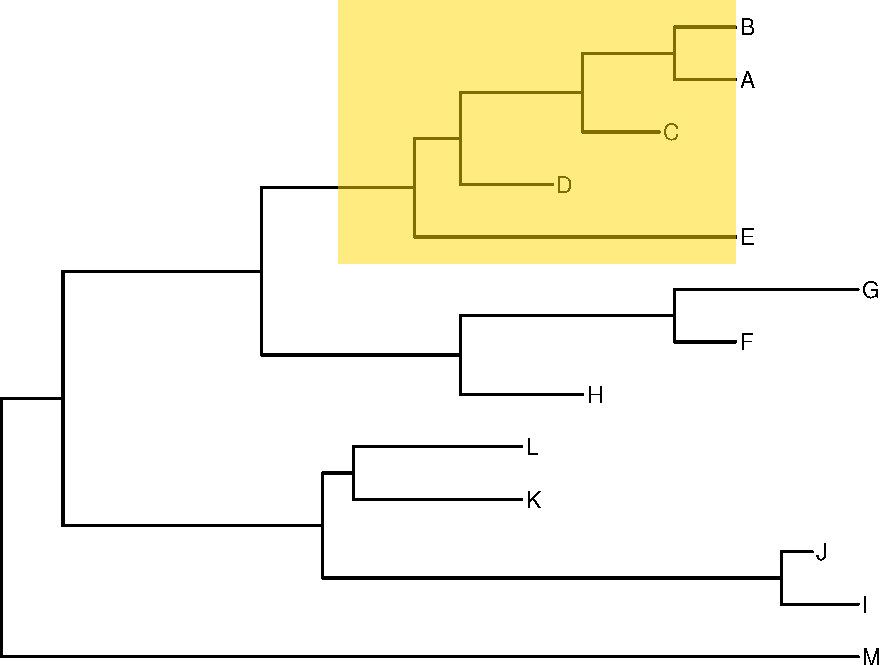
\includegraphics{bookdown-demo_files/figure-latex/unnamed-chunk-34-1} \end{center}

If you prefer, you can manually set the colour for all points. Be aware
of the difference here! In the code below, the difference is that colour
here is outside of the mapping argument. This means that the colour
doesn't display any real information but does change the aesthetic of
the plot.

\begin{Shaded}
\begin{Highlighting}[]
\KeywordTok{ggplot}\NormalTok{(}\DataTypeTok{data =}\NormalTok{ primate.data) }\OperatorTok{+}
\StringTok{  }\KeywordTok{geom_point}\NormalTok{(}\DataTypeTok{mapping =} \KeywordTok{aes}\NormalTok{(}\DataTypeTok{x =} \KeywordTok{log10}\NormalTok{(AdultBodyMass_g), }\DataTypeTok{y =}\NormalTok{ GestationLen_d),}
             \DataTypeTok{colour =} \StringTok{"green"}\NormalTok{)}
\end{Highlighting}
\end{Shaded}

\begin{center}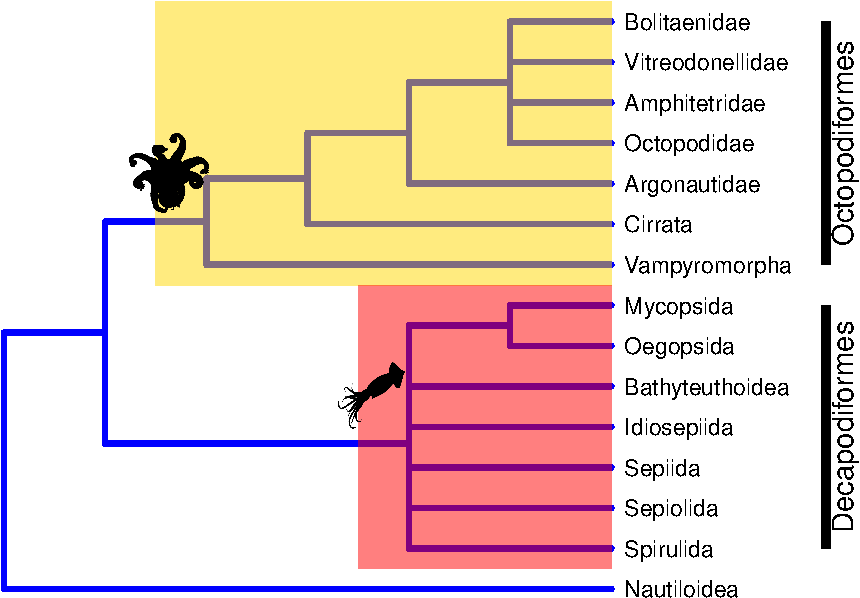
\includegraphics{bookdown-demo_files/figure-latex/unnamed-chunk-35-1} \end{center}

Let's clean up the plot with some axis labels.

\begin{Shaded}
\begin{Highlighting}[]
\KeywordTok{ggplot}\NormalTok{(}\DataTypeTok{data =}\NormalTok{ primate.data) }\OperatorTok{+}
\StringTok{  }\KeywordTok{geom_point}\NormalTok{(}\DataTypeTok{mapping =} \KeywordTok{aes}\NormalTok{(}\DataTypeTok{x =} \KeywordTok{log10}\NormalTok{(AdultBodyMass_g), }\DataTypeTok{y =}\NormalTok{ GestationLen_d,}
                           \DataTypeTok{colour =}\NormalTok{ Family)) }\OperatorTok{+}
\StringTok{  }\KeywordTok{labs}\NormalTok{(}\DataTypeTok{x =} \StringTok{"Log Body Mass"}\NormalTok{, }\DataTypeTok{y =} \StringTok{"Gestation Length"}\NormalTok{)}
\end{Highlighting}
\end{Shaded}

\begin{center}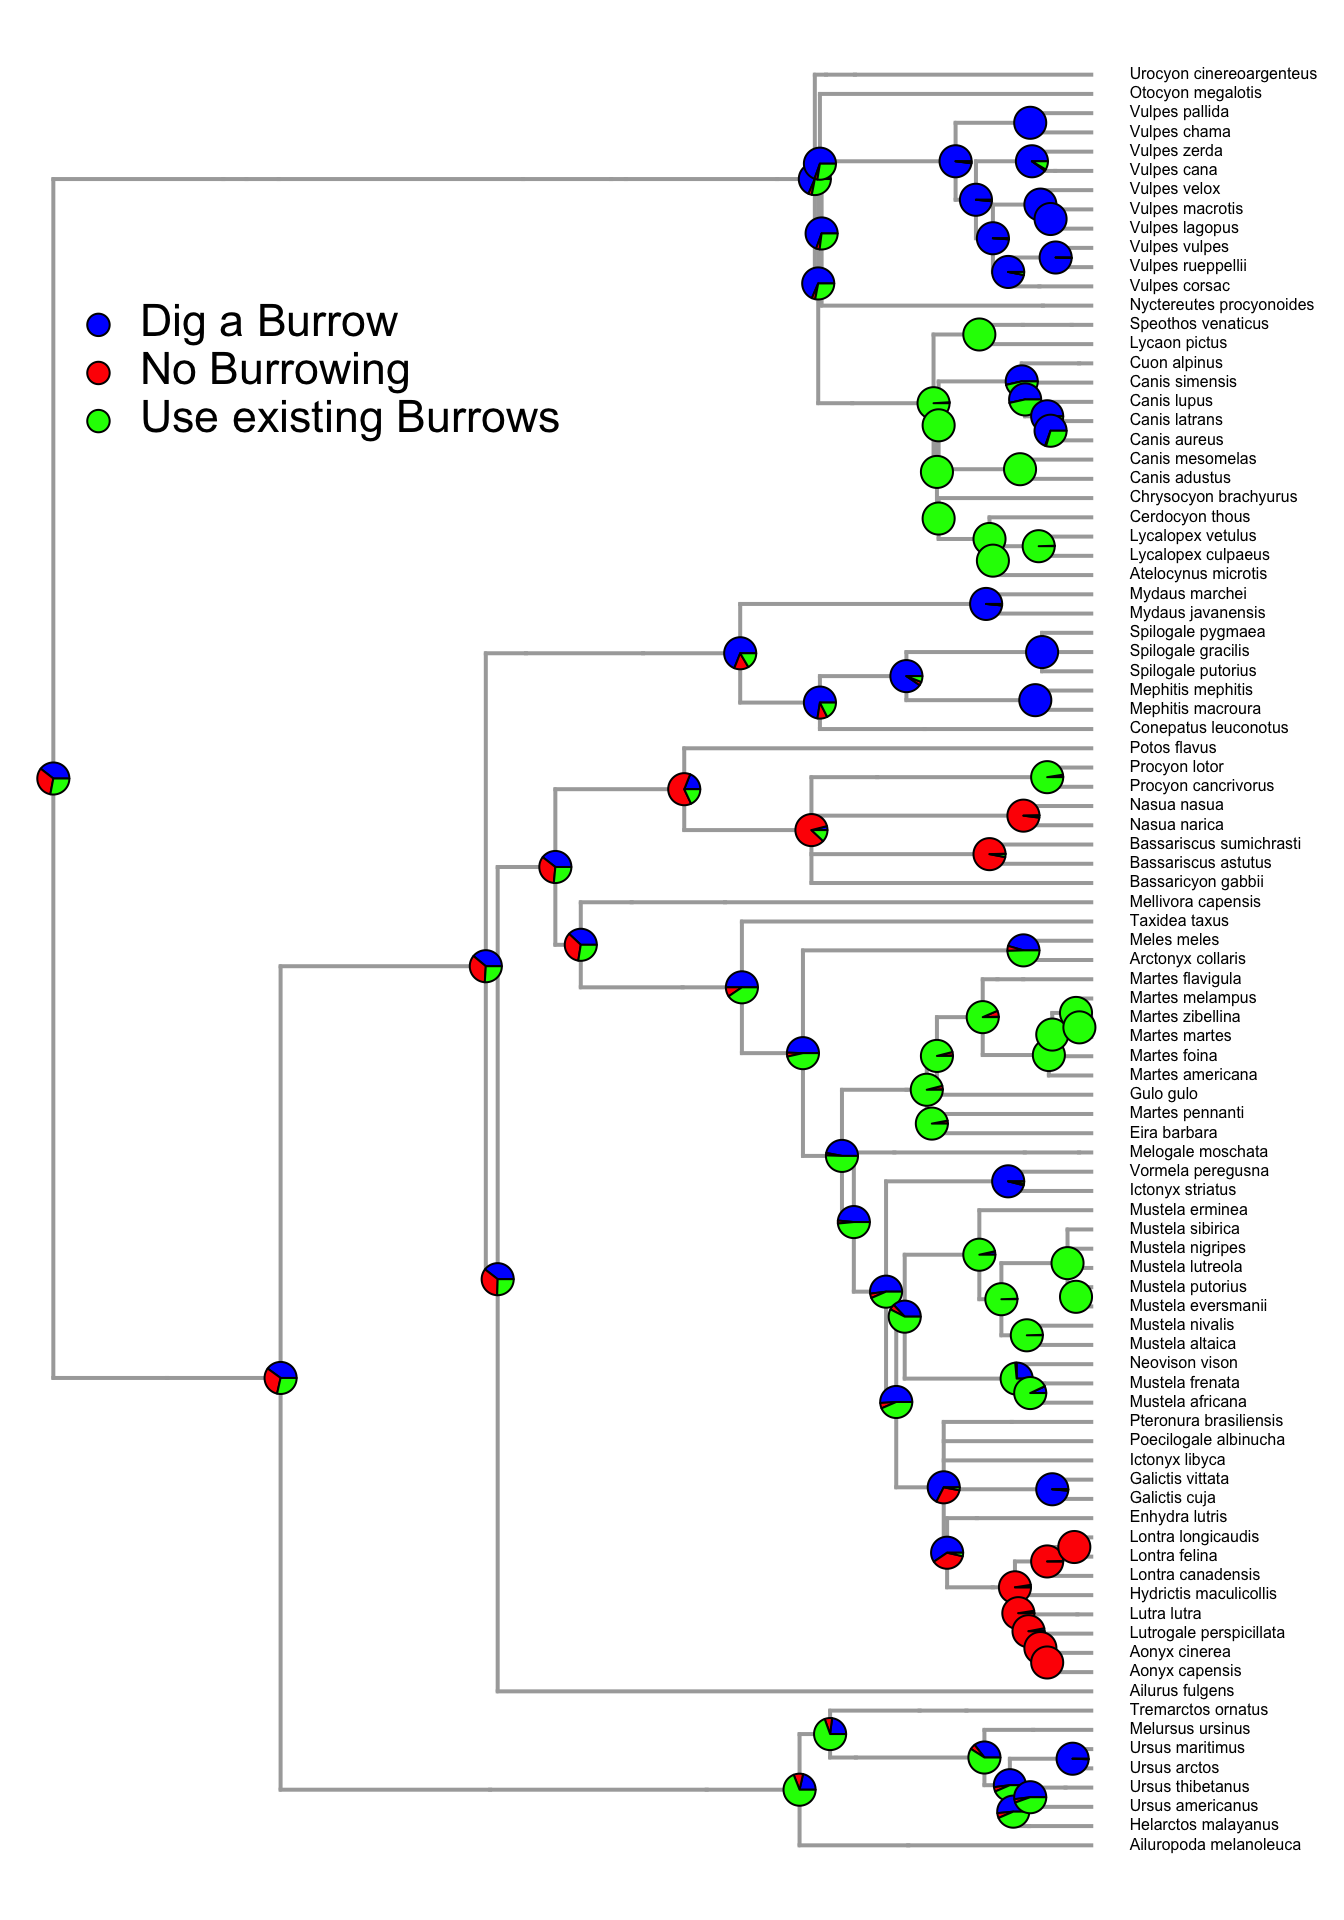
\includegraphics{bookdown-demo_files/figure-latex/unnamed-chunk-36-1} \end{center}

\section{Linear Regression}\label{linear-regression}

To see if body mass and gestation length are related, the best way to go
would seem to be a linear regression. The funtion to perform an ordinary
least squares linear regression is lm(). The first argument is our
model, stating in this case that body mass predicts gestation length.
Then we specify the data object to tell R where to find the data.

\begin{Shaded}
\begin{Highlighting}[]
\NormalTok{m1 <-}\StringTok{ }\KeywordTok{lm}\NormalTok{(GestationLen_d }\OperatorTok{~}\StringTok{ }\KeywordTok{log10}\NormalTok{(AdultBodyMass_g), }\DataTypeTok{data =}\NormalTok{ primate.data)}
\end{Highlighting}
\end{Shaded}

You should now see a new object (m1) in your environment. This contains
the output of your regression analysis and to view it, we can use the
summary function.

\begin{Shaded}
\begin{Highlighting}[]
\KeywordTok{summary}\NormalTok{(m1)}
\end{Highlighting}
\end{Shaded}

\begin{verbatim}

Call:
lm(formula = GestationLen_d ~ log10(AdultBodyMass_g), data = primate.data)

Residuals:
    Min      1Q  Median      3Q     Max 
-66.665 -15.762  -3.987  16.869  67.121 

Coefficients:
                       Estimate Std. Error t value Pr(>|t|)    
(Intercept)              31.775     13.927   2.281   0.0249 *  
log10(AdultBodyMass_g)   38.319      4.031   9.505 3.37e-15 ***
---
Signif. codes:  0 '***' 0.001 '**' 0.01 '*' 0.05 '.' 0.1 ' ' 1

Residual standard error: 27.31 on 89 degrees of freedom
Multiple R-squared:  0.5038,    Adjusted R-squared:  0.4982 
F-statistic: 90.35 on 1 and 89 DF,  p-value: 3.374e-15
\end{verbatim}

The key parts of our output are the coefficients table and the three
lines of output below which contain the R\textsuperscript{2} value.
Here, it's telling us that our model is a significant fit to the data as
we might expect. Also, the mid-range R\textsuperscript{2} (0.50) is what
we'd expect given the spread of data in the plot.

We can also plot this line with ggplot with the following code. There
are some key differences here. Most importantly, I've specified x and y
in ggplot rather than geom\_point. I've then added the function
geom\_smooth amd used the method ``lm'' to specify that I want a linear
model plotted. The reason I did this is quite simple; I Googled it and
the hive-mind of R users on the internet told me to.

\begin{Shaded}
\begin{Highlighting}[]
\KeywordTok{ggplot}\NormalTok{(}\DataTypeTok{data =}\NormalTok{ primate.data, }\KeywordTok{aes}\NormalTok{(}\DataTypeTok{x =} \KeywordTok{log10}\NormalTok{(AdultBodyMass_g), }\DataTypeTok{y =}\NormalTok{ GestationLen_d)) }\OperatorTok{+}
\StringTok{  }\KeywordTok{geom_point}\NormalTok{() }\OperatorTok{+}\StringTok{ }
\StringTok{  }\KeywordTok{geom_smooth}\NormalTok{(}\DataTypeTok{method =} \StringTok{"lm"}\NormalTok{, }\DataTypeTok{se =} \OtherTok{FALSE}\NormalTok{)}
\end{Highlighting}
\end{Shaded}

\begin{center}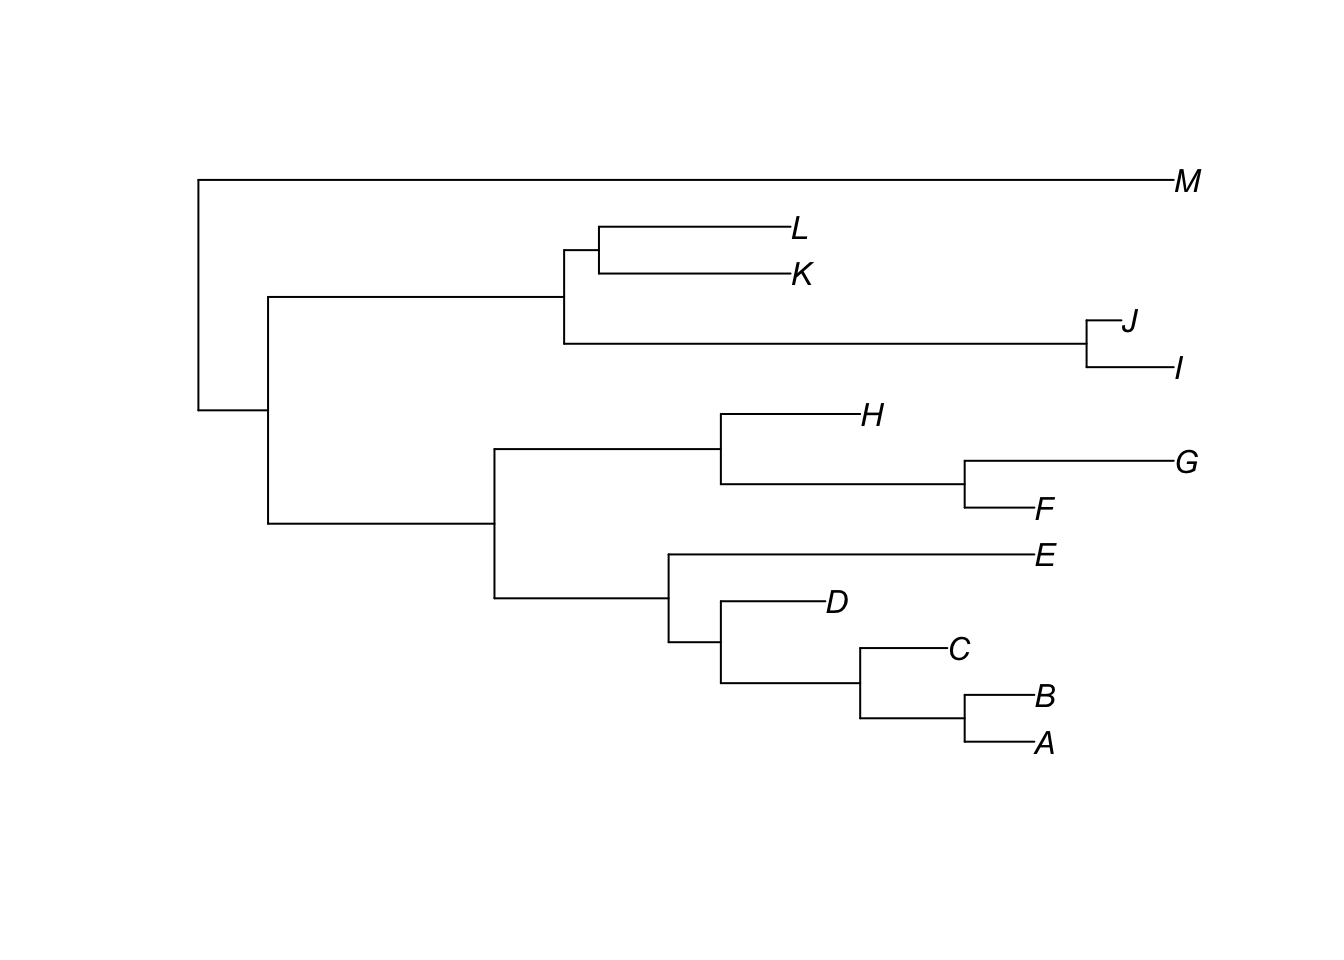
\includegraphics{bookdown-demo_files/figure-latex/unnamed-chunk-39-1} \end{center}

\section{Trees and Phylogenetic
Signal}\label{trees-and-phylogenetic-signal}

As you know, the fact that comparative data points are not statistically
independent is a problem for these kind of analyses. Therefore we need
to run a phylogenetically corrected analysis.

\subsection{Phylogenetic signal}\label{phylogenetic-signal}

Importantly, you need to understand the concept of phylogenetic signal
which is defined as \emph{the tendency for closely related species to
resemble each other more than distantly related species}.

For example, body mass is (usually) a trait with a strong phylogenetic
signal. What this means in primates is that although there is a broad
range of body sizes from a few tens of grams up to around 200kg, the
distribution of body masses closely follows the pattern of relatedness.
Large primates like orangutan, gorillas, chimps and humans are all
closely related for example.

The degree of phylogenetic signal in a trait is often described using
the scaling parameter \(\lambda\). \(\lambda\) varies between 0 and 1
and is used to multiply the internal branch lengths so that the tree
describes the pattern of variation in the trait.

For example, take the case on the left, where \(\lambda = 1\). In this
case the tree is untransformed because the variation in the trait
follows the structure of the tree. On the right, where \(\lambda = 0\),
all the internal branch lengths have been multiplied by 0 and therefore
collapsed. This ``star phylogeny'' describes a pattern of variation in
which the trait varies at random with respect to the phylogeny. The
trait is not equal across the tree but rather the variation in the trait
does not correlate to the pattern of relatedness.

\begin{center}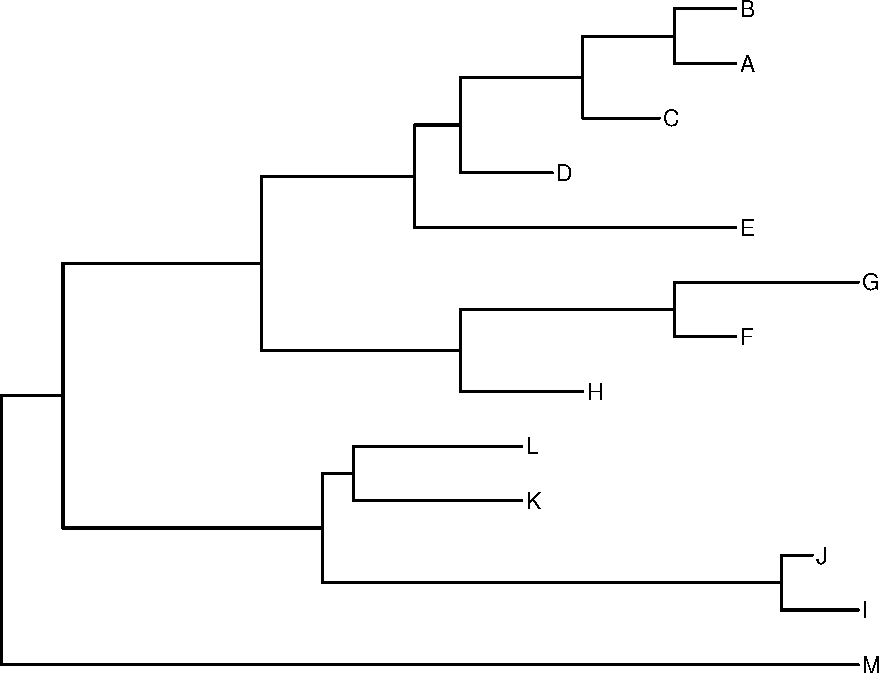
\includegraphics{bookdown-demo_files/figure-latex/unnamed-chunk-40-1} \end{center}

\subsection{caper}\label{caper}

Let's run through some examples. There are a few packages that can run
phylogenetic regressions in R but the one I usually go with is called
caper (Comparative Analysis of Phylogenetics and Evolution in R). So
first we'll need to load caper.

\begin{Shaded}
\begin{Highlighting}[]
\KeywordTok{library}\NormalTok{(caper)}
\end{Highlighting}
\end{Shaded}

Now we can load up our phylogeny using read.nexus from the ape package.

\begin{Shaded}
\begin{Highlighting}[]
\NormalTok{primate.tree <-}\StringTok{ }\KeywordTok{read.nexus}\NormalTok{(}\StringTok{"primate_tree.nex"}\NormalTok{)}
\end{Highlighting}
\end{Shaded}

The regression command in caper (along with some other functions)
requires the data and tree to be combined in a comparative data object.
This type of objectis simply a tree and comparative data set
concatenated and is created using the function ``comparative.data''. We
need to specify the tree object, data object, column name in the data
where species names are stored and whether we want a variance-covariance
matrix included (we do).

\begin{Shaded}
\begin{Highlighting}[]
\NormalTok{primates <-}\StringTok{ }\KeywordTok{comparative.data}\NormalTok{(}\DataTypeTok{phy =}\NormalTok{ primate.tree,     }\CommentTok{#Our tree}
                             \DataTypeTok{data =}\NormalTok{ primate.data,    }\CommentTok{#Our data}
                             \DataTypeTok{names.col =}\NormalTok{ Binomial,   }\CommentTok{#Data column with the species names}
                             \DataTypeTok{vcv =} \OtherTok{TRUE}\NormalTok{,             }\CommentTok{#Variance-covariance matrix}
                             \DataTypeTok{na.omit =} \OtherTok{FALSE}\NormalTok{,        }\CommentTok{#We don't want to drop missing data}
                             \DataTypeTok{warn.dropped =} \OtherTok{TRUE}\NormalTok{)}
\end{Highlighting}
\end{Shaded}

\begin{verbatim}
Warning in comparative.data(phy = primate.tree, data = primate.data,
names.col = Binomial, : Data dropped in compiling comparative data object
\end{verbatim}

This warning message isn't really a problem. If you look at the tree and
data I provided, you'll see that the tree has about 200 species but the
data contains data for only 91. Therefore we expected R to drop some
species when compiling the comparative data object. In fact, we asked it
warn us if it did so!

We can inspect the structure of the comparative data object using str if
necessary. You should see that the object contains both the tree and the
data. Either one of these (pruned from the larger objects we specified)
can be extracted again if needed.

\begin{Shaded}
\begin{Highlighting}[]
\KeywordTok{str}\NormalTok{(primates)}
\end{Highlighting}
\end{Shaded}

\begin{verbatim}
List of 7
 $ phy      :List of 5
  ..$ edge       : int [1:163, 1:2] 84 85 86 87 88 89 90 91 92 93 ...
  ..$ edge.length: num [1:163] 4.95 17.69 19.65 8.12 4.82 ...
  ..$ Nnode      : int 81
  ..$ tip.label  : chr [1:83] "Cercopithecus_ascanius" "Cercopithecus_cephus" "Cercopithecus_mitis" "Cercopithecus_neglectus" ...
  ..$ node.label : int [1:81] 84 85 86 87 88 89 90 91 92 93 ...
  ..- attr(*, "class")= chr "phylo"
  ..- attr(*, "order")= chr "cladewise"
 $ data     :'data.frame':  83 obs. of  7 variables:
  ..$ Order          : Factor w/ 1 level "Primates": 1 1 1 1 1 1 1 1 1 1 ...
  ..$ Family         : Factor w/ 15 levels "Aotidae","Atelidae",..: 4 4 4 4 4 4 4 5 5 6 ...
  ..$ AdultBodyMass_g: num [1:83] 3540 3445 5041 5325 5257 ...
  ..$ GestationLen_d : num [1:83] 148 170 138 172 170 ...
  ..$ HomeRange_km2  : num [1:83] 0.16 0.24 0.1 0.06 1.15 ...
  ..$ MaxLongevity_m : num [1:83] 340 276 325 316 276 ...
  ..$ SocialGroupSize: num [1:83] 26.3 11 16 4.5 16 28 91.2 1 1 1 ...
 $ data.name: chr "primate.data"
 $ phy.name : chr "primate.tree"
 $ dropped  :List of 2
  ..$ tips          : chr [1:143] "Allenopithecus_nigroviridis" "Cercopithecus_cephus_cephus" "Cercopithecus_cephus_ngottoensis" "Cercopithecus_diana" ...
  ..$ unmatched.rows: chr [1:8] "Cercopithecus_campbelli" "Cercopithecus_pogonias" "Chiropotes_albinasus" "Chiropotes_satanas" ...
 $ vcv      : 'VCV.array' num [1:83, 1:83] 72.3 69 64 62.4 64 ...
  ..- attr(*, "dimnames")=List of 2
  .. ..$ : chr [1:83] "Cercopithecus_ascanius" "Cercopithecus_cephus" "Cercopithecus_mitis" "Cercopithecus_neglectus" ...
  .. ..$ : chr [1:83] "Cercopithecus_ascanius" "Cercopithecus_cephus" "Cercopithecus_mitis" "Cercopithecus_neglectus" ...
 $ vcv.dim  : num 2
 - attr(*, "class")= chr "comparative.data"
\end{verbatim}

\subsection{Estimating Phylogenetic
Signal}\label{estimating-phylogenetic-signal}

Let's estimate the phylogenetic signal of gestation length in primates.
The key is to remember that we need to call our comparative data object
and not the data file we loaded up at the start. We're running the trait
on its own (hence the ``\textasciitilde{} 1'') and estimating lambda by
maximum likelihood.

\begin{Shaded}
\begin{Highlighting}[]
\NormalTok{signal <-}\StringTok{ }\KeywordTok{pgls}\NormalTok{(}\KeywordTok{log10}\NormalTok{(GestationLen_d) }\OperatorTok{~}\StringTok{ }\DecValTok{1}\NormalTok{,}
               \DataTypeTok{data =}\NormalTok{ primates,}
               \DataTypeTok{lambda =} \StringTok{"ML"}\NormalTok{)}
\end{Highlighting}
\end{Shaded}

The object ``signal'' should have appeared in your environment now. We
can inspect the object using the ever-useful summary function.

\begin{Shaded}
\begin{Highlighting}[]
\KeywordTok{summary}\NormalTok{(signal)}
\end{Highlighting}
\end{Shaded}

\begin{verbatim}

Call:
pgls(formula = log10(GestationLen_d) ~ 1, data = primates, lambda = "ML")

Residuals:
      Min        1Q    Median        3Q       Max 
-0.035946 -0.007060 -0.001217  0.008039  0.049662 

Branch length transformations:

kappa  [Fix]  : 1.000
lambda [ ML]  : 0.957
   lower bound : 0.000, p = < 2.22e-16
   upper bound : 1.000, p = 0.050633
   95.0% CI   : (0.879, NA)
delta  [Fix]  : 1.000

Coefficients:
            Estimate Std. Error t value  Pr(>|t|)    
(Intercept) 2.175175   0.051457  42.272 < 2.2e-16 ***
---
Signif. codes:  0 '***' 0.001 '**' 0.01 '*' 0.05 '.' 0.1 ' ' 1

Residual standard error: 0.01462 on 82 degrees of freedom
Multiple R-squared:     0,  Adjusted R-squared:     0 
F-statistic:   NaN on 0 and 82 DF,  p-value: NA 
\end{verbatim}

This output has a lot in common with a basic regression output. That's
because it is one! We used the pgls function which performs a regression
with phylogenetic correction. Because we included no predictors, the
value of \(\lambda\) we estimate here corresponds only to this one
trait.

The key part for us is the \textit{Branch length transformations}
section of the output. \(\kappa\) and \(\delta\) are fixed at 1 and so
we aren't concerned with those for now. \(\lambda\) is estimated at
0.957. That's a pretty strong phylogenetic signal.

We also have lower bound and upper bound tests. We can see that
\(\lambda\) is significantly different from the lower bound of 0 (p
\textless{} 2.2 x 10\textsuperscript{-16}). This isn't surprising at
all!

The upper bound test shows us that \(\lambda\) is (narrowly) not
significantly different from 1 (p = 0.051). This means that we can
assume that gestation length has evolved by Brownian Motion, in which
case \(\lambda\) would equal 1 and the variation in trait would simply
reflect the pattern of relatedness amongst species.

\section{Phylogenetic Regression}\label{phylogenetic-regression}

Now let's have a go at performing a PGLS regression!

Let's say we have an idea that larger species of primate have longer
gestations. Our plot seems to back this up but how strong is this
relationship?

\begin{center}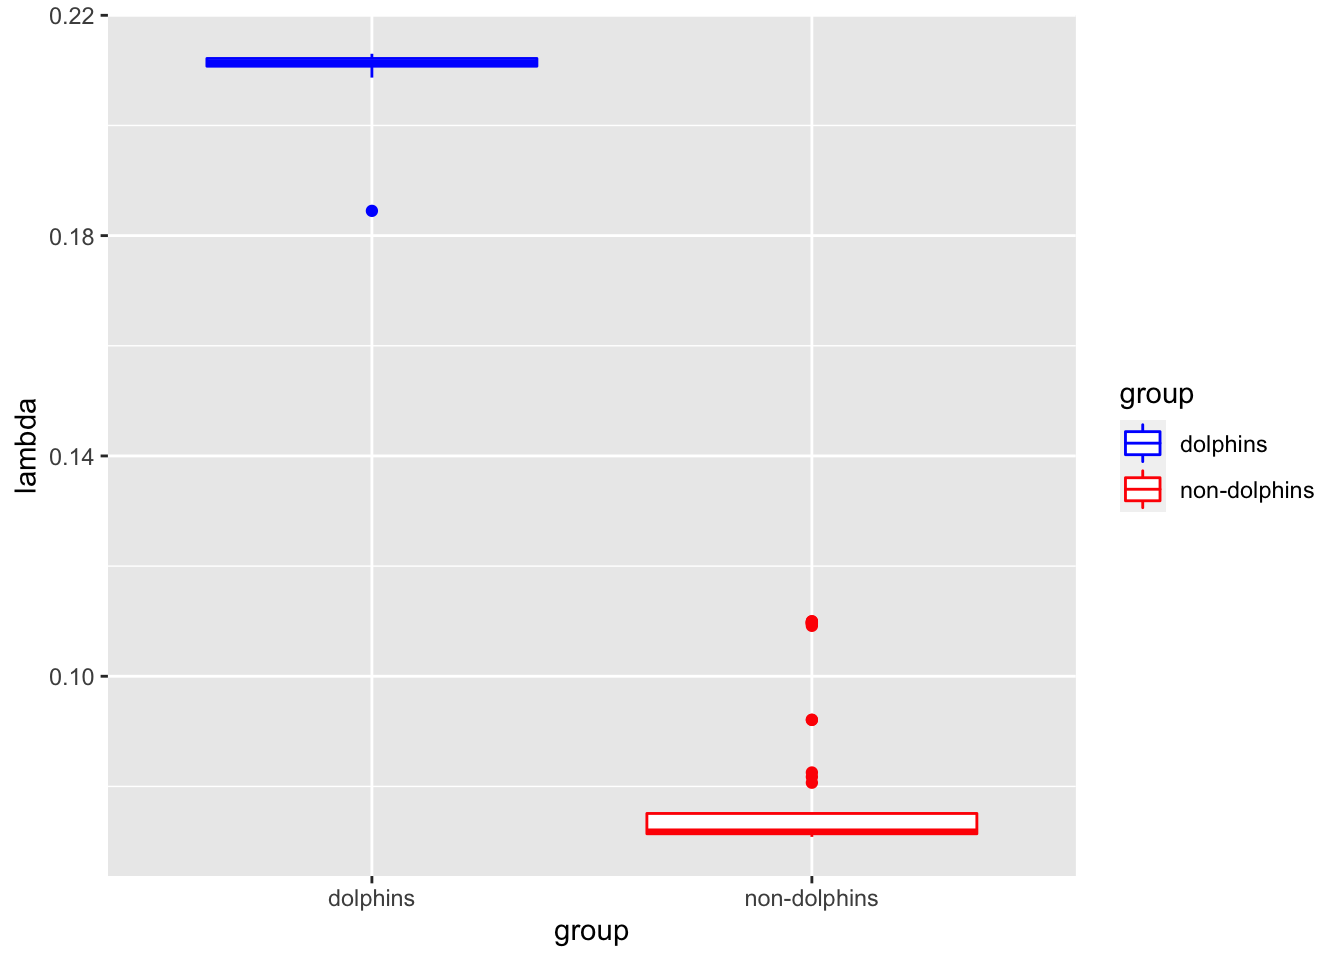
\includegraphics{bookdown-demo_files/figure-latex/unnamed-chunk-47-1} \end{center}

We found earlier that there does seem to be a relationship but ordinary
least squares linear regression can't really be relied upon in this
situation. This is because of the statistical non-independence of data
points due to shared evolutionary history!

A phylogenetic generalised least squares regression (PGLS) uses a
covariance matrix to correct the analysis for this statistical
non-independence. Put simply, the PGLS assumes the residuals are more
similar in more closely related species rather than being randomly
distributed as in linear regression.

As you've already seen, the function we need here is ``pgls''. The model
is constructed exactly as before but this time, we need to construct a
full model. We'll be estimating \(\lambda\) by maximum likelihood again.

\begin{Shaded}
\begin{Highlighting}[]
\NormalTok{m2 <-}\StringTok{ }\KeywordTok{pgls}\NormalTok{(GestationLen_d }\OperatorTok{~}\StringTok{ }\KeywordTok{log10}\NormalTok{(AdultBodyMass_g), }\DataTypeTok{data =}\NormalTok{ primates, }\DataTypeTok{lambda =} \StringTok{"ML"}\NormalTok{)}
\end{Highlighting}
\end{Shaded}

The summary function gets the key details we need.

\begin{Shaded}
\begin{Highlighting}[]
\KeywordTok{summary}\NormalTok{(m2)}
\end{Highlighting}
\end{Shaded}

\begin{verbatim}

Call:
pgls(formula = GestationLen_d ~ log10(AdultBodyMass_g), data = primates, 
    lambda = "ML")

Residuals:
     Min       1Q   Median       3Q      Max 
-13.0979  -2.4301  -0.8407   1.7269   6.9863 

Branch length transformations:

kappa  [Fix]  : 1.000
lambda [ ML]  : 0.805
   lower bound : 0.000, p = 2.6579e-12
   upper bound : 1.000, p = 1.042e-06
   95.0% CI   : (0.607, 0.920)
delta  [Fix]  : 1.000

Coefficients:
                       Estimate Std. Error t value  Pr(>|t|)    
(Intercept)             53.6444    20.9100  2.5655   0.01215 *  
log10(AdultBodyMass_g)  33.7532     5.8487  5.7710 1.394e-07 ***
---
Signif. codes:  0 '***' 0.001 '**' 0.01 '*' 0.05 '.' 0.1 ' ' 1

Residual standard error: 3.513 on 81 degrees of freedom
Multiple R-squared: 0.2914, Adjusted R-squared: 0.2826 
F-statistic:  33.3 on 1 and 81 DF,  p-value: 1.394e-07 
\end{verbatim}

As you can see, our model is a significant fit to the data (F = 33.3,
R\textsuperscript{2} = 0.29, p = 1.39 x 10\textsuperscript{-7}). More
importantly, We've confirmed that body size has a positive effect on
gestation length (\(\beta\) = 33.75, s.e. = 5.85, p = 1.39 x
10\textsuperscript{-7}). Time to plot!

A brief note here. The syntax to get ggplot to do this is a little more
complex than base graphics (where we can just use abline(m2)!). Here
I've plotted both the OLS (blue) and PGLS (red) lines so you can see how
they differ.

\begin{Shaded}
\begin{Highlighting}[]
\NormalTok{primates}\OperatorTok{$}\NormalTok{data }\OperatorTok
\StringTok{  }\KeywordTok{mutate}\NormalTok{(}\DataTypeTok{my_model =} \KeywordTok{predict}\NormalTok{(m2)) }\OperatorTok
\StringTok{  }\KeywordTok{ggplot}\NormalTok{() }\OperatorTok{+}
\StringTok{  }\KeywordTok{geom_point}\NormalTok{(}\KeywordTok{aes}\NormalTok{(}\KeywordTok{log10}\NormalTok{(AdultBodyMass_g), GestationLen_d)) }\OperatorTok{+}
\StringTok{  }\KeywordTok{geom_line}\NormalTok{(}\KeywordTok{aes}\NormalTok{(}\KeywordTok{log10}\NormalTok{(AdultBodyMass_g), my_model), }
            \DataTypeTok{colour =} \StringTok{"red"}\NormalTok{, }\DataTypeTok{lwd =} \DecValTok{1}\NormalTok{) }\OperatorTok{+}
\StringTok{  }\KeywordTok{geom_smooth}\NormalTok{(}\KeywordTok{aes}\NormalTok{(}\KeywordTok{log10}\NormalTok{(AdultBodyMass_g), GestationLen_d), }
              \DataTypeTok{method =} \StringTok{'lm'}\NormalTok{, }\DataTypeTok{se =} \OtherTok{FALSE}\NormalTok{) }\OperatorTok{+}
\StringTok{  }\KeywordTok{labs}\NormalTok{(}\DataTypeTok{x =} \StringTok{"Log Body Mass"}\NormalTok{, }\DataTypeTok{y =} \StringTok{"Gestation Length"}\NormalTok{) }\OperatorTok{+}
\StringTok{  }\KeywordTok{geom_text}\NormalTok{(}\DataTypeTok{x =} \DecValTok{2}\NormalTok{, }\DataTypeTok{y =} \DecValTok{230}\NormalTok{, }\DataTypeTok{label =} \StringTok{"PGLS"}\NormalTok{, }\DataTypeTok{colour =} \StringTok{"red"}\NormalTok{, }\DataTypeTok{size =} \DecValTok{4}\NormalTok{) }\OperatorTok{+}
\StringTok{  }\KeywordTok{geom_text}\NormalTok{(}\DataTypeTok{x =} \DecValTok{2}\NormalTok{, }\DataTypeTok{y =} \DecValTok{218}\NormalTok{, }\DataTypeTok{label =} \StringTok{"OLS"}\NormalTok{, }\DataTypeTok{colour =} \StringTok{"blue"}\NormalTok{, }\DataTypeTok{size =} \DecValTok{4}\NormalTok{)}
\end{Highlighting}
\end{Shaded}

\begin{center}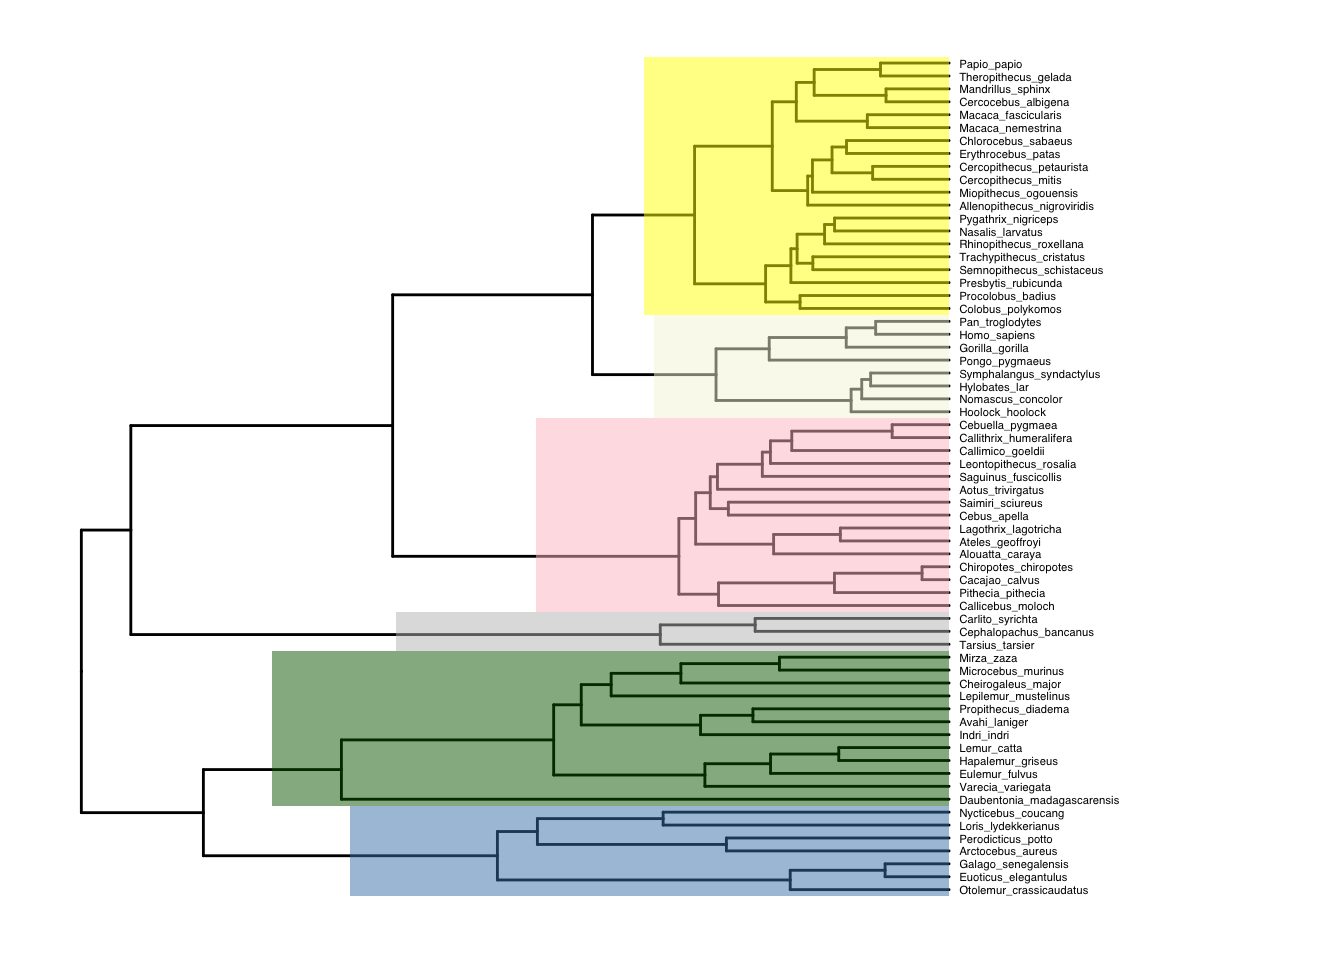
\includegraphics{bookdown-demo_files/figure-latex/unnamed-chunk-51-1} \end{center}

\subsection{Model Checking}\label{model-checking}

That's the basic model run nicely. Now, we need to run some diagnostic
checks. We should start with the likelihood surface of \(\lambda\) since
we estimated it by maximum likelihood.

We begin by using the pgls.profile function to extract the likelihoods
and then simply plot them. I'm going to keep it simple by using base
graphics for this. What we are looking for is a single peak around our
estimated value. If we get a flat surface or multiple peaks, there might
be an issue somewhere.

\begin{Shaded}
\begin{Highlighting}[]
\NormalTok{lambda.profile <-}\StringTok{ }\KeywordTok{pgls.profile}\NormalTok{(m2, }\DataTypeTok{which =} \StringTok{"lambda"}\NormalTok{)}
\KeywordTok{plot}\NormalTok{(lambda.profile)}
\end{Highlighting}
\end{Shaded}

\begin{center}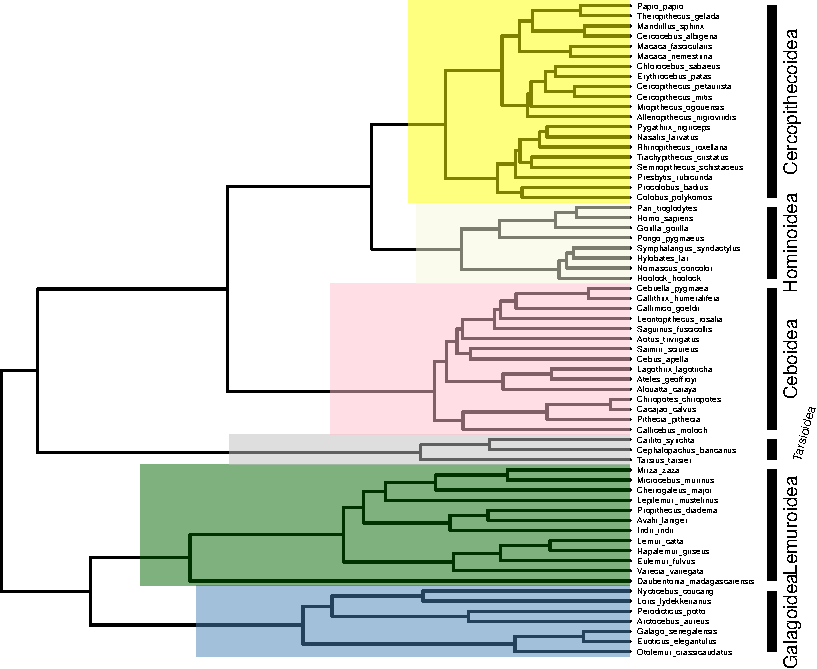
\includegraphics{bookdown-demo_files/figure-latex/unnamed-chunk-52-1} \end{center}

This plot describes the log likelihood of \(\lambda\) across its
possible range of values (0 - 1). We can clearly see that the likelihood
is highest around a single point around 0.8. Check back against the
model output earlier to see if this is what we would expect.

Next we need to identify any outliers in the model residuals. The first
step here is to extract the residuals from the model, making sure to
tell R that we want the phylogenetic residuals. The model output of pgls
actually stores both phylogenetic and non-phylogenetic residuals. We can
then standardise the residuals by dividing through by the square root of
the variance.

\begin{Shaded}
\begin{Highlighting}[]
\NormalTok{res <-}\StringTok{ }\KeywordTok{residuals}\NormalTok{(m2, }\DataTypeTok{phylo =} \OtherTok{TRUE}\NormalTok{)}
\NormalTok{res <-}\StringTok{ }\NormalTok{res}\OperatorTok{/}\KeywordTok{sqrt}\NormalTok{(}\KeywordTok{var}\NormalTok{(res))[}\DecValTok{1}\NormalTok{]}
\end{Highlighting}
\end{Shaded}

The general rule is that any standardised residual with an absolute
value greater than 3 is an outlier and needs to be removed from any
analysis. Here, I'm just assigning the species names to the res object
so we can tell which species are the outliers (if any).

\begin{Shaded}
\begin{Highlighting}[]
\KeywordTok{rownames}\NormalTok{(res) <-}\StringTok{ }\KeywordTok{rownames}\NormalTok{(m2}\OperatorTok{$}\NormalTok{residuals)}
\KeywordTok{rownames}\NormalTok{(res)[}\KeywordTok{abs}\NormalTok{(res)}\OperatorTok{>}\DecValTok{3}\NormalTok{]}
\end{Highlighting}
\end{Shaded}

\begin{verbatim}
[1] "Microcebus_murinus" "Prolemur_simus"    
\end{verbatim}

Outliers! Maybe they're causing problems and maybe they aren't. We need
to check that by re-running our analysis without them. A simple line of
code will take our existing comparative data object and drop out the
named outliers.

\begin{Shaded}
\begin{Highlighting}[]
\NormalTok{primates.nooutliers <-}\StringTok{ }\NormalTok{primates[}\OperatorTok{-}\KeywordTok{which}\NormalTok{(}\KeywordTok{abs}\NormalTok{(res)}\OperatorTok{>}\DecValTok{3}\NormalTok{),]}
\end{Highlighting}
\end{Shaded}

Now simply re-run the model, remembering to direct R to the new data
object.

\begin{Shaded}
\begin{Highlighting}[]
\NormalTok{m3 <-}\StringTok{ }\KeywordTok{pgls}\NormalTok{(GestationLen_d }\OperatorTok{~}\StringTok{ }\KeywordTok{log10}\NormalTok{(AdultBodyMass_g),}
           \DataTypeTok{data =}\NormalTok{ primates.nooutliers, }
           \DataTypeTok{lambda =} \StringTok{"ML"}\NormalTok{)}
\KeywordTok{summary}\NormalTok{(m3)}
\end{Highlighting}
\end{Shaded}

\begin{verbatim}

Call:
pgls(formula = GestationLen_d ~ log10(AdultBodyMass_g), data = primates.nooutliers, 
    lambda = "ML")

Residuals:
     Min       1Q   Median       3Q      Max 
-10.2217  -2.0473  -0.4166   1.3041  11.2824 

Branch length transformations:

kappa  [Fix]  : 1.000
lambda [ ML]  : 0.800
   lower bound : 0.000, p = 1.6399e-11
   upper bound : 1.000, p = 1.2064e-06
   95.0% CI   : (0.595, 0.918)
delta  [Fix]  : 1.000

Coefficients:
                       Estimate Std. Error t value  Pr(>|t|)    
(Intercept)             54.8023    21.1816  2.5873   0.01151 *  
log10(AdultBodyMass_g)  33.3672     5.9418  5.6156 2.815e-07 ***
---
Signif. codes:  0 '***' 0.001 '**' 0.01 '*' 0.05 '.' 0.1 ' ' 1

Residual standard error: 3.53 on 79 degrees of freedom
Multiple R-squared: 0.2853, Adjusted R-squared: 0.2762 
F-statistic: 31.54 on 1 and 79 DF,  p-value: 2.815e-07 
\end{verbatim}

The results have barely changed. So it seems that although those two
lemurs were outliers, they weren't effecting the analysis too much.
Let's check for outliers in this new model.

\begin{Shaded}
\begin{Highlighting}[]
\NormalTok{res <-}\StringTok{ }\KeywordTok{residuals}\NormalTok{(m3, }\DataTypeTok{phylo =} \OtherTok{TRUE}\NormalTok{)}
\NormalTok{res <-}\StringTok{ }\NormalTok{res}\OperatorTok{/}\KeywordTok{sqrt}\NormalTok{(}\KeywordTok{var}\NormalTok{(res))[}\DecValTok{1}\NormalTok{]}
\KeywordTok{rownames}\NormalTok{(res) <-}\StringTok{ }\KeywordTok{rownames}\NormalTok{(m3}\OperatorTok{$}\NormalTok{residuals)}
\KeywordTok{rownames}\NormalTok{(res)[}\KeywordTok{abs}\NormalTok{(res)}\OperatorTok{>}\DecValTok{3}\NormalTok{]}
\end{Highlighting}
\end{Shaded}

\begin{verbatim}
[1] "Microcebus_rufus"
\end{verbatim}

Another one! Don't worry. This can happen. We need to drop the new
outlier again to run the same checks.

Finally, we can check the diagnostic plots of the model. I've included
some lines to help arrange the plots. To view the plots for model
diagnostics, we can simply plot the model object!

\begin{Shaded}
\begin{Highlighting}[]
\NormalTok{par.default <-}\StringTok{ }\KeywordTok{par}\NormalTok{(}\DataTypeTok{no.readonly =}\NormalTok{ T) }\CommentTok{#Save default plotting parameters}
\KeywordTok{par}\NormalTok{(}\DataTypeTok{mfrow=}\KeywordTok{c}\NormalTok{(}\DecValTok{2}\NormalTok{,}\DecValTok{2}\NormalTok{)) }\CommentTok{#Set the plot window to show 4 different plots}

\KeywordTok{plot}\NormalTok{(m3)}
\end{Highlighting}
\end{Shaded}

\begin{center}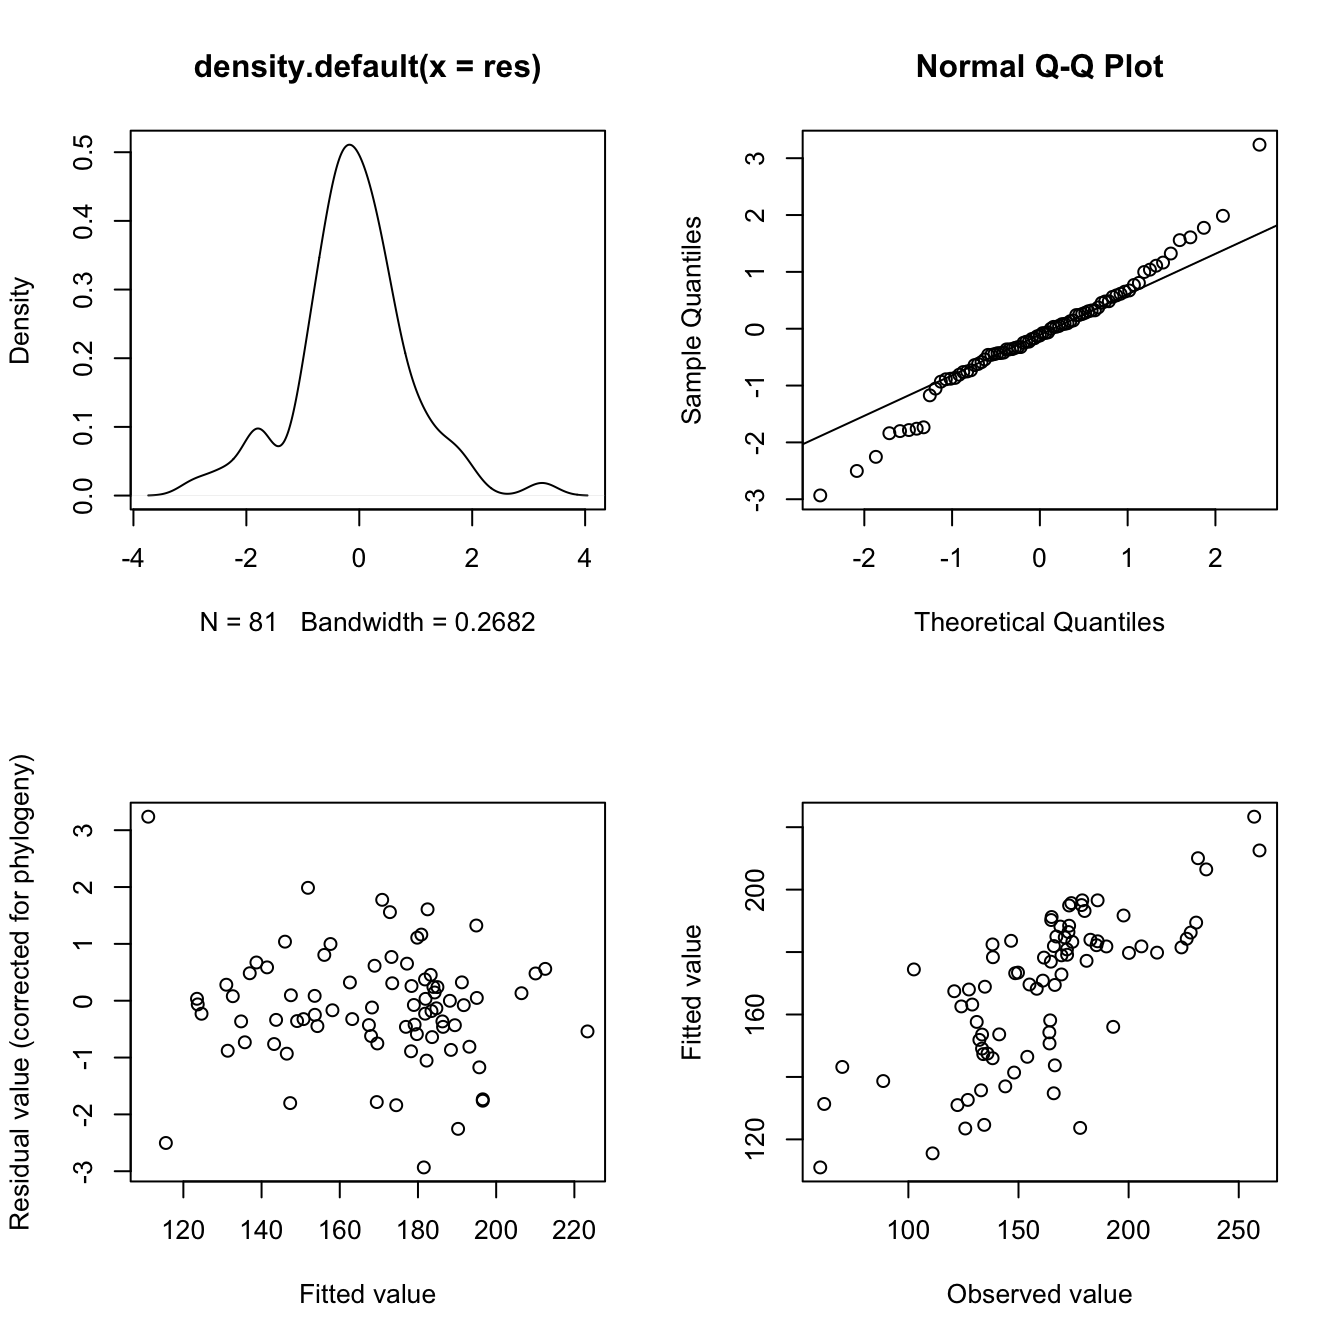
\includegraphics{bookdown-demo_files/figure-latex/unnamed-chunk-58-1} \end{center}

\begin{Shaded}
\begin{Highlighting}[]
\KeywordTok{par}\NormalTok{(par.default) }\CommentTok{#Reset plot window to default}
\end{Highlighting}
\end{Shaded}

The top left panel shows the distribution of our residuals. We can see a
bump near +3. That will be our outlier that needs to be dropped before
we proceed any further. The top right plot closely approximates a
straight line so that's good. The bottom left shows no real pattern
which is also good. The bottom right graph should show a correlation
(and it seems to) with the points more or less equally scattered above
and below the 45\textsuperscript{o} diagonal. Along that line, the
observed and fitted values would be exactly equal.

\section{Conclusion}\label{conclusion}

So that's how to perform a simple PGLS analysis. This kind of analysis
is great for attempting make causal connections between traits of extant
species, thus inferring a connection over evolutionary history. For
example, we hypothesised that the reason some primates have longer
gestation periods is that they have larger body sizes and the pgls
confirmed our suspicion. More complex regressions can include multpile
predictors and that's what we'll look at next.

By the way, always make sure to check your models for outliers! In this
analysis the gray mouse lemur was an outlier and we had to drop it.
Outliers like this can throw off your analysis. If we hadn't checked, we
would have presented the analysis in a paper and then had it invalidated
when someone checked up on it. Fortunately in this case, the outliers
didn't really change the outcome so the gray mouse lemur is off the
hook. Look how relieved he is!

\begin{center}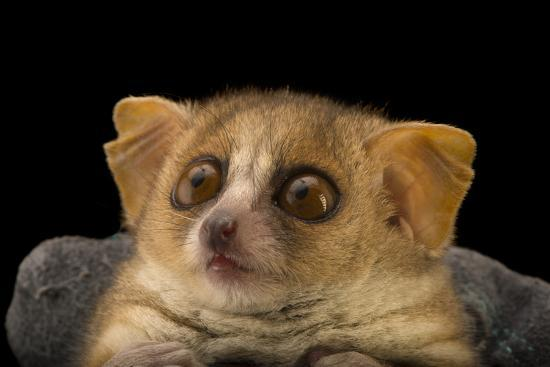
\includegraphics[width=7.64in]{~/Google Drive/University of Liverpool/GitHub Stuff/bookdownCRG/Images/mouse lemur} \end{center}

\bibliography{book.bib,packages.bib}

\end{document}
